% Options for packages loaded elsewhere
\PassOptionsToPackage{unicode}{hyperref}
\PassOptionsToPackage{hyphens}{url}
\PassOptionsToPackage{dvipsnames,svgnames,x11names}{xcolor}
%
\documentclass[
  letterpaper,
  DIV=11,
  numbers=noendperiod]{scrartcl}

\usepackage{amsmath,amssymb}
\usepackage{iftex}
\ifPDFTeX
  \usepackage[T1]{fontenc}
  \usepackage[utf8]{inputenc}
  \usepackage{textcomp} % provide euro and other symbols
\else % if luatex or xetex
  \usepackage{unicode-math}
  \defaultfontfeatures{Scale=MatchLowercase}
  \defaultfontfeatures[\rmfamily]{Ligatures=TeX,Scale=1}
\fi
\usepackage{lmodern}
\ifPDFTeX\else  
    % xetex/luatex font selection
\fi
% Use upquote if available, for straight quotes in verbatim environments
\IfFileExists{upquote.sty}{\usepackage{upquote}}{}
\IfFileExists{microtype.sty}{% use microtype if available
  \usepackage[]{microtype}
  \UseMicrotypeSet[protrusion]{basicmath} % disable protrusion for tt fonts
}{}
\makeatletter
\@ifundefined{KOMAClassName}{% if non-KOMA class
  \IfFileExists{parskip.sty}{%
    \usepackage{parskip}
  }{% else
    \setlength{\parindent}{0pt}
    \setlength{\parskip}{6pt plus 2pt minus 1pt}}
}{% if KOMA class
  \KOMAoptions{parskip=half}}
\makeatother
\usepackage{xcolor}
\setlength{\emergencystretch}{3em} % prevent overfull lines
\setcounter{secnumdepth}{-\maxdimen} % remove section numbering
% Make \paragraph and \subparagraph free-standing
\ifx\paragraph\undefined\else
  \let\oldparagraph\paragraph
  \renewcommand{\paragraph}[1]{\oldparagraph{#1}\mbox{}}
\fi
\ifx\subparagraph\undefined\else
  \let\oldsubparagraph\subparagraph
  \renewcommand{\subparagraph}[1]{\oldsubparagraph{#1}\mbox{}}
\fi

\usepackage{color}
\usepackage{fancyvrb}
\newcommand{\VerbBar}{|}
\newcommand{\VERB}{\Verb[commandchars=\\\{\}]}
\DefineVerbatimEnvironment{Highlighting}{Verbatim}{commandchars=\\\{\}}
% Add ',fontsize=\small' for more characters per line
\usepackage{framed}
\definecolor{shadecolor}{RGB}{241,243,245}
\newenvironment{Shaded}{\begin{snugshade}}{\end{snugshade}}
\newcommand{\AlertTok}[1]{\textcolor[rgb]{0.68,0.00,0.00}{#1}}
\newcommand{\AnnotationTok}[1]{\textcolor[rgb]{0.37,0.37,0.37}{#1}}
\newcommand{\AttributeTok}[1]{\textcolor[rgb]{0.40,0.45,0.13}{#1}}
\newcommand{\BaseNTok}[1]{\textcolor[rgb]{0.68,0.00,0.00}{#1}}
\newcommand{\BuiltInTok}[1]{\textcolor[rgb]{0.00,0.23,0.31}{#1}}
\newcommand{\CharTok}[1]{\textcolor[rgb]{0.13,0.47,0.30}{#1}}
\newcommand{\CommentTok}[1]{\textcolor[rgb]{0.37,0.37,0.37}{#1}}
\newcommand{\CommentVarTok}[1]{\textcolor[rgb]{0.37,0.37,0.37}{\textit{#1}}}
\newcommand{\ConstantTok}[1]{\textcolor[rgb]{0.56,0.35,0.01}{#1}}
\newcommand{\ControlFlowTok}[1]{\textcolor[rgb]{0.00,0.23,0.31}{#1}}
\newcommand{\DataTypeTok}[1]{\textcolor[rgb]{0.68,0.00,0.00}{#1}}
\newcommand{\DecValTok}[1]{\textcolor[rgb]{0.68,0.00,0.00}{#1}}
\newcommand{\DocumentationTok}[1]{\textcolor[rgb]{0.37,0.37,0.37}{\textit{#1}}}
\newcommand{\ErrorTok}[1]{\textcolor[rgb]{0.68,0.00,0.00}{#1}}
\newcommand{\ExtensionTok}[1]{\textcolor[rgb]{0.00,0.23,0.31}{#1}}
\newcommand{\FloatTok}[1]{\textcolor[rgb]{0.68,0.00,0.00}{#1}}
\newcommand{\FunctionTok}[1]{\textcolor[rgb]{0.28,0.35,0.67}{#1}}
\newcommand{\ImportTok}[1]{\textcolor[rgb]{0.00,0.46,0.62}{#1}}
\newcommand{\InformationTok}[1]{\textcolor[rgb]{0.37,0.37,0.37}{#1}}
\newcommand{\KeywordTok}[1]{\textcolor[rgb]{0.00,0.23,0.31}{#1}}
\newcommand{\NormalTok}[1]{\textcolor[rgb]{0.00,0.23,0.31}{#1}}
\newcommand{\OperatorTok}[1]{\textcolor[rgb]{0.37,0.37,0.37}{#1}}
\newcommand{\OtherTok}[1]{\textcolor[rgb]{0.00,0.23,0.31}{#1}}
\newcommand{\PreprocessorTok}[1]{\textcolor[rgb]{0.68,0.00,0.00}{#1}}
\newcommand{\RegionMarkerTok}[1]{\textcolor[rgb]{0.00,0.23,0.31}{#1}}
\newcommand{\SpecialCharTok}[1]{\textcolor[rgb]{0.37,0.37,0.37}{#1}}
\newcommand{\SpecialStringTok}[1]{\textcolor[rgb]{0.13,0.47,0.30}{#1}}
\newcommand{\StringTok}[1]{\textcolor[rgb]{0.13,0.47,0.30}{#1}}
\newcommand{\VariableTok}[1]{\textcolor[rgb]{0.07,0.07,0.07}{#1}}
\newcommand{\VerbatimStringTok}[1]{\textcolor[rgb]{0.13,0.47,0.30}{#1}}
\newcommand{\WarningTok}[1]{\textcolor[rgb]{0.37,0.37,0.37}{\textit{#1}}}

\providecommand{\tightlist}{%
  \setlength{\itemsep}{0pt}\setlength{\parskip}{0pt}}\usepackage{longtable,booktabs,array}
\usepackage{calc} % for calculating minipage widths
% Correct order of tables after \paragraph or \subparagraph
\usepackage{etoolbox}
\makeatletter
\patchcmd\longtable{\par}{\if@noskipsec\mbox{}\fi\par}{}{}
\makeatother
% Allow footnotes in longtable head/foot
\IfFileExists{footnotehyper.sty}{\usepackage{footnotehyper}}{\usepackage{footnote}}
\makesavenoteenv{longtable}
\usepackage{graphicx}
\makeatletter
\def\maxwidth{\ifdim\Gin@nat@width>\linewidth\linewidth\else\Gin@nat@width\fi}
\def\maxheight{\ifdim\Gin@nat@height>\textheight\textheight\else\Gin@nat@height\fi}
\makeatother
% Scale images if necessary, so that they will not overflow the page
% margins by default, and it is still possible to overwrite the defaults
% using explicit options in \includegraphics[width, height, ...]{}
\setkeys{Gin}{width=\maxwidth,height=\maxheight,keepaspectratio}
% Set default figure placement to htbp
\makeatletter
\def\fps@figure{htbp}
\makeatother

\usepackage{fontspec}
\usepackage{multirow}
\usepackage{multicol}
\usepackage{colortbl}
\usepackage{hhline}
\newlength\Oldarrayrulewidth
\newlength\Oldtabcolsep
\usepackage{longtable}
\usepackage{array}
\usepackage{hyperref}
\usepackage{float}
\usepackage{wrapfig}
\KOMAoption{captions}{tableheading}
\makeatletter
\makeatother
\makeatletter
\makeatother
\makeatletter
\@ifpackageloaded{caption}{}{\usepackage{caption}}
\AtBeginDocument{%
\ifdefined\contentsname
  \renewcommand*\contentsname{Table of contents}
\else
  \newcommand\contentsname{Table of contents}
\fi
\ifdefined\listfigurename
  \renewcommand*\listfigurename{List of Figures}
\else
  \newcommand\listfigurename{List of Figures}
\fi
\ifdefined\listtablename
  \renewcommand*\listtablename{List of Tables}
\else
  \newcommand\listtablename{List of Tables}
\fi
\ifdefined\figurename
  \renewcommand*\figurename{Figure}
\else
  \newcommand\figurename{Figure}
\fi
\ifdefined\tablename
  \renewcommand*\tablename{Table}
\else
  \newcommand\tablename{Table}
\fi
}
\@ifpackageloaded{float}{}{\usepackage{float}}
\floatstyle{ruled}
\@ifundefined{c@chapter}{\newfloat{codelisting}{h}{lop}}{\newfloat{codelisting}{h}{lop}[chapter]}
\floatname{codelisting}{Listing}
\newcommand*\listoflistings{\listof{codelisting}{List of Listings}}
\makeatother
\makeatletter
\@ifpackageloaded{caption}{}{\usepackage{caption}}
\@ifpackageloaded{subcaption}{}{\usepackage{subcaption}}
\makeatother
\makeatletter
\@ifpackageloaded{tcolorbox}{}{\usepackage[skins,breakable]{tcolorbox}}
\makeatother
\makeatletter
\@ifundefined{shadecolor}{\definecolor{shadecolor}{rgb}{.97, .97, .97}}
\makeatother
\makeatletter
\makeatother
\makeatletter
\makeatother
\ifLuaTeX
  \usepackage{selnolig}  % disable illegal ligatures
\fi
\IfFileExists{bookmark.sty}{\usepackage{bookmark}}{\usepackage{hyperref}}
\IfFileExists{xurl.sty}{\usepackage{xurl}}{} % add URL line breaks if available
\urlstyle{same} % disable monospaced font for URLs
\hypersetup{
  pdftitle={Assignment 1: Decision trees and cost-effectiveness},
  pdfauthor={YOUR NAME HERE},
  colorlinks=true,
  linkcolor={blue},
  filecolor={Maroon},
  citecolor={Blue},
  urlcolor={Blue},
  pdfcreator={LaTeX via pandoc}}

\title{Assignment 1: Decision trees and cost-effectiveness}
\author{YOUR NAME HERE}
\date{2023-08-10}

\begin{document}
\maketitle
\ifdefined\Shaded\renewenvironment{Shaded}{\begin{tcolorbox}[sharp corners, interior hidden, boxrule=0pt, borderline west={3pt}{0pt}{shadecolor}, enhanced, frame hidden, breakable]}{\end{tcolorbox}}\fi

\renewcommand*\contentsname{Table of contents}
{
\hypersetup{linkcolor=}
\setcounter{tocdepth}{3}
\tableofcontents
}
\begin{Shaded}
\begin{Highlighting}[]
\CommentTok{\# Load packages}
\CommentTok{\#.  Use install.packages("XXXX") if you don\textquotesingle{}t have any of these installed}
\FunctionTok{library}\NormalTok{(rdecision) }\CommentTok{\#decision trees}
\FunctionTok{library}\NormalTok{(flextable) }\CommentTok{\#Formatting tables to display (https://davidgohel.github.io/flextable/reference/index.html)}
\FunctionTok{library}\NormalTok{(ggplot2) }\CommentTok{\#Plotting}
\FunctionTok{library}\NormalTok{(readxl) }\CommentTok{\#for read\_excel()}
\FunctionTok{library}\NormalTok{(dplyr) }\CommentTok{\# I use mutate at one point}
\end{Highlighting}
\end{Shaded}

\begin{verbatim}

Attaching package: 'dplyr'
\end{verbatim}

\begin{verbatim}
The following objects are masked from 'package:stats':

    filter, lag
\end{verbatim}

\begin{verbatim}
The following objects are masked from 'package:base':

    intersect, setdiff, setequal, union
\end{verbatim}

\begin{Shaded}
\begin{Highlighting}[]
\FunctionTok{theme\_set}\NormalTok{(}\FunctionTok{theme\_bw}\NormalTok{()) }\CommentTok{\#Makes ggplots look better}
\end{Highlighting}
\end{Shaded}

\hypertarget{section-1-decision-trees}{%
\section{Section 1: Decision trees}\label{section-1-decision-trees}}

We'll use the
\href{https://cran.r-project.org/web/packages/rdecision/index.html}{rdecision
package} to develop and visualize decision trees. There are a few
vignettes on the CRAN page.
\href{https://cran.rstudio.com/web/packages/rdecision/vignettes/DT00-DecisionTreeTutorial.html}{This
introductory one} will probably be sufficient for you to understand how
we are using the package in this assignment.

\hypertarget{a-expected-value-calculations}{%
\subsection{1a Expected value
calculations}\label{a-expected-value-calculations}}

This first code chunk is just an example; you don't need to edit it.
Here, using the rdecision package, I have created a decision tree,
visualized it, and ``rolled it back'' to calculate the expected cost and
QALYs associated with the two alternatives. Review it carefully, because
in 1b, you'll do similar calculations for a different decision tree.

\begin{Shaded}
\begin{Highlighting}[]
\CommentTok{\# Decision problem: Should we use diet or exercise to reduce chance of needing a stent in a high{-}risk population?}

\CommentTok{\# Parameters}
\NormalTok{c\_diet }\OtherTok{\textless{}{-}} \DecValTok{50} \CommentTok{\#cost of diet}
\NormalTok{c\_exercise }\OtherTok{\textless{}{-}} \DecValTok{750} \CommentTok{\#cost of exercise}
\NormalTok{c\_stent }\OtherTok{\textless{}{-}} \DecValTok{5000} \CommentTok{\#cost of a stent}
\NormalTok{u\_stent }\OtherTok{\textless{}{-}} \FloatTok{0.75} \CommentTok{\#utility of getting a stent (relative to 1.0)}
\NormalTok{p\_stent\_diet }\OtherTok{\textless{}{-}}\NormalTok{ (}\DecValTok{68} \SpecialCharTok{{-}} \DecValTok{12}\NormalTok{)}\SpecialCharTok{/}\DecValTok{68} \CommentTok{\#probability needing stent if we diet}
\NormalTok{p\_stent\_exercise }\OtherTok{\textless{}{-}}\NormalTok{ (}\DecValTok{58} \SpecialCharTok{{-}} \DecValTok{18}\NormalTok{)}\SpecialCharTok{/}\DecValTok{58} \CommentTok{\#probability of needing a stent if we exercise}

\CommentTok{\#Build model using rdecision package}

\CommentTok{\#Create decision and chance nodes}
\NormalTok{decision\_node }\OtherTok{\textless{}{-}}\NormalTok{ DecisionNode}\SpecialCharTok{$}\FunctionTok{new}\NormalTok{(}\StringTok{"Diet or exercise"}\NormalTok{)}
\NormalTok{chance\_node\_diet }\OtherTok{\textless{}{-}}\NormalTok{ ChanceNode}\SpecialCharTok{$}\FunctionTok{new}\NormalTok{(}\StringTok{"Stent?"}\NormalTok{)}
\NormalTok{chance\_node\_exercise }\OtherTok{\textless{}{-}}\NormalTok{ ChanceNode}\SpecialCharTok{$}\FunctionTok{new}\NormalTok{(}\StringTok{"Stent?"}\NormalTok{)}

\CommentTok{\#Create leaf nodes}
\NormalTok{leaf\_node\_diet\_no\_stent }\OtherTok{\textless{}{-}}\NormalTok{ LeafNode}\SpecialCharTok{$}\FunctionTok{new}\NormalTok{(}\StringTok{"No stent"}\NormalTok{)}
\NormalTok{leaf\_node\_diet\_stent }\OtherTok{\textless{}{-}}\NormalTok{ LeafNode}\SpecialCharTok{$}\FunctionTok{new}\NormalTok{(}\StringTok{"Stent"}\NormalTok{, }\AttributeTok{utility =}\NormalTok{ u\_stent)}
\NormalTok{leaf\_node\_exercise\_no\_stent }\OtherTok{\textless{}{-}}\NormalTok{ LeafNode}\SpecialCharTok{$}\FunctionTok{new}\NormalTok{(}\StringTok{"No stent"}\NormalTok{)}
\NormalTok{leaf\_node\_exercise\_stent }\OtherTok{\textless{}{-}}\NormalTok{ LeafNode}\SpecialCharTok{$}\FunctionTok{new}\NormalTok{(}\StringTok{"Stent"}\NormalTok{, }\AttributeTok{utility =}\NormalTok{ u\_stent)}

\CommentTok{\#Create \textquotesingle{}actions\textquotesingle{}, paths from your decision node(s)}
\NormalTok{action\_diet }\OtherTok{\textless{}{-}}\NormalTok{ Action}\SpecialCharTok{$}\FunctionTok{new}\NormalTok{(}
\NormalTok{  decision\_node, chance\_node\_diet, }\AttributeTok{cost =}\NormalTok{ c\_diet, }\AttributeTok{label =} \StringTok{"Diet"}
\NormalTok{)}
\NormalTok{action\_exercise }\OtherTok{\textless{}{-}}\NormalTok{ Action}\SpecialCharTok{$}\FunctionTok{new}\NormalTok{(}
\NormalTok{  decision\_node, chance\_node\_exercise, }\AttributeTok{cost =}\NormalTok{ c\_exercise, }\AttributeTok{label =} \StringTok{"Exercise"}
\NormalTok{)}

\CommentTok{\#Create \textquotesingle{}reactions\textquotesingle{}, paths from your chance node(s)}
\NormalTok{reaction\_diet\_success }\OtherTok{\textless{}{-}}\NormalTok{ Reaction}\SpecialCharTok{$}\FunctionTok{new}\NormalTok{(}
\NormalTok{  chance\_node\_diet, leaf\_node\_diet\_no\_stent, }
  \AttributeTok{p =} \DecValTok{1}\SpecialCharTok{{-}}\NormalTok{p\_stent\_diet, }\AttributeTok{cost =} \FloatTok{0.0}\NormalTok{, }\AttributeTok{label =} \StringTok{"Did not need stent"}\NormalTok{)}

\NormalTok{reaction\_diet\_failure }\OtherTok{\textless{}{-}}\NormalTok{ Reaction}\SpecialCharTok{$}\FunctionTok{new}\NormalTok{(}
\NormalTok{  chance\_node\_diet, leaf\_node\_diet\_stent, }
  \AttributeTok{p =}\NormalTok{ p\_stent\_diet, }\AttributeTok{cost =}\NormalTok{ c\_stent, }\AttributeTok{label =} \StringTok{"Needed stent"}\NormalTok{)}

\NormalTok{reaction\_exercise\_success }\OtherTok{\textless{}{-}}\NormalTok{ Reaction}\SpecialCharTok{$}\FunctionTok{new}\NormalTok{(}
\NormalTok{  chance\_node\_exercise, leaf\_node\_exercise\_no\_stent, }
  \AttributeTok{p =} \DecValTok{1}\SpecialCharTok{{-}}\NormalTok{p\_stent\_exercise, }\AttributeTok{cost =} \FloatTok{0.0}\NormalTok{, }\AttributeTok{label =} \StringTok{"Did not need stent"}\NormalTok{)}

\NormalTok{reaction\_exercise\_failure }\OtherTok{\textless{}{-}}\NormalTok{ Reaction}\SpecialCharTok{$}\FunctionTok{new}\NormalTok{(}
\NormalTok{  chance\_node\_exercise, leaf\_node\_exercise\_stent, }
  \AttributeTok{p =}\NormalTok{ p\_stent\_exercise, }\AttributeTok{cost =} \FloatTok{5000.0}\NormalTok{, }\AttributeTok{label =} \StringTok{"Needed stent"}\NormalTok{)}

\CommentTok{\#Create, draw, and evaluate the tree}
\NormalTok{DT1 }\OtherTok{\textless{}{-}}\NormalTok{ DecisionTree}\SpecialCharTok{$}\FunctionTok{new}\NormalTok{(}
  \AttributeTok{V =} \FunctionTok{list}\NormalTok{(decision\_node, }\CommentTok{\#verticies (nodes)}
\NormalTok{           chance\_node\_diet, }
\NormalTok{           chance\_node\_exercise, }
\NormalTok{           leaf\_node\_diet\_no\_stent, }
\NormalTok{           leaf\_node\_diet\_stent, }
\NormalTok{           leaf\_node\_exercise\_no\_stent, }
\NormalTok{           leaf\_node\_exercise\_stent),}
  \AttributeTok{E =} \FunctionTok{list}\NormalTok{(action\_diet, }\CommentTok{\#edges (paths between nodes)}
\NormalTok{           action\_exercise,}
\NormalTok{           reaction\_diet\_success,}
\NormalTok{           reaction\_diet\_failure,}
\NormalTok{           reaction\_exercise\_success,}
\NormalTok{           reaction\_exercise\_failure)}
\NormalTok{)}

\NormalTok{DT1}\SpecialCharTok{$}\FunctionTok{draw}\NormalTok{() }\CommentTok{\#Plot it}
\end{Highlighting}
\end{Shaded}

\begin{figure}[H]

{\centering 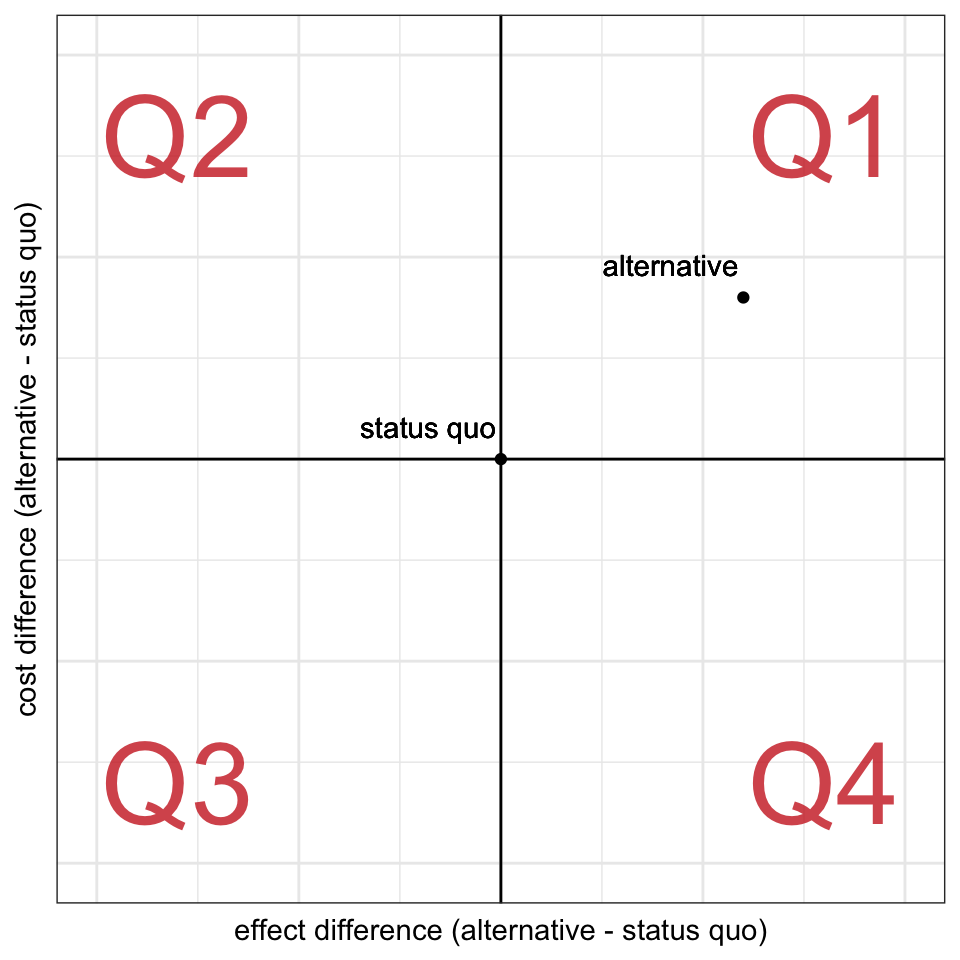
\includegraphics{assign1_trees_cea_files/figure-pdf/unnamed-chunk-2-1.pdf}

}

\end{figure}

\begin{Shaded}
\begin{Highlighting}[]
\NormalTok{DT1\_evaluation }\OtherTok{\textless{}{-}}\NormalTok{ DT1}\SpecialCharTok{$}\FunctionTok{evaluate}\NormalTok{() }\CommentTok{\#calculate it}
\NormalTok{DT1\_evaluation }\SpecialCharTok{|\textgreater{}} \FunctionTok{flextable}\NormalTok{()}
\end{Highlighting}
\end{Shaded}

\global\setlength{\Oldarrayrulewidth}{\arrayrulewidth}

\global\setlength{\Oldtabcolsep}{\tabcolsep}

\setlength{\tabcolsep}{0pt}

\renewcommand*{\arraystretch}{1.5}



\providecommand{\ascline}[3]{\noalign{\global\arrayrulewidth #1}\arrayrulecolor[HTML]{#2}\cline{#3}}

\begin{longtable*}[c]{|p{0.75in}|p{0.75in}|p{0.75in}|p{0.75in}|p{0.75in}|p{0.75in}|p{0.75in}}



\ascline{1.5pt}{666666}{1-7}

\multicolumn{1}{>{\raggedright}m{\dimexpr 0.75in+0\tabcolsep}}{\textcolor[HTML]{000000}{\fontsize{11}{11}\selectfont{Diet.or.exercise}}} & \multicolumn{1}{>{\raggedleft}m{\dimexpr 0.75in+0\tabcolsep}}{\textcolor[HTML]{000000}{\fontsize{11}{11}\selectfont{Run}}} & \multicolumn{1}{>{\raggedleft}m{\dimexpr 0.75in+0\tabcolsep}}{\textcolor[HTML]{000000}{\fontsize{11}{11}\selectfont{Probability}}} & \multicolumn{1}{>{\raggedleft}m{\dimexpr 0.75in+0\tabcolsep}}{\textcolor[HTML]{000000}{\fontsize{11}{11}\selectfont{Cost}}} & \multicolumn{1}{>{\raggedleft}m{\dimexpr 0.75in+0\tabcolsep}}{\textcolor[HTML]{000000}{\fontsize{11}{11}\selectfont{Benefit}}} & \multicolumn{1}{>{\raggedleft}m{\dimexpr 0.75in+0\tabcolsep}}{\textcolor[HTML]{000000}{\fontsize{11}{11}\selectfont{Utility}}} & \multicolumn{1}{>{\raggedleft}m{\dimexpr 0.75in+0\tabcolsep}}{\textcolor[HTML]{000000}{\fontsize{11}{11}\selectfont{QALY}}} \\

\ascline{1.5pt}{666666}{1-7}\endfirsthead 

\ascline{1.5pt}{666666}{1-7}

\multicolumn{1}{>{\raggedright}m{\dimexpr 0.75in+0\tabcolsep}}{\textcolor[HTML]{000000}{\fontsize{11}{11}\selectfont{Diet.or.exercise}}} & \multicolumn{1}{>{\raggedleft}m{\dimexpr 0.75in+0\tabcolsep}}{\textcolor[HTML]{000000}{\fontsize{11}{11}\selectfont{Run}}} & \multicolumn{1}{>{\raggedleft}m{\dimexpr 0.75in+0\tabcolsep}}{\textcolor[HTML]{000000}{\fontsize{11}{11}\selectfont{Probability}}} & \multicolumn{1}{>{\raggedleft}m{\dimexpr 0.75in+0\tabcolsep}}{\textcolor[HTML]{000000}{\fontsize{11}{11}\selectfont{Cost}}} & \multicolumn{1}{>{\raggedleft}m{\dimexpr 0.75in+0\tabcolsep}}{\textcolor[HTML]{000000}{\fontsize{11}{11}\selectfont{Benefit}}} & \multicolumn{1}{>{\raggedleft}m{\dimexpr 0.75in+0\tabcolsep}}{\textcolor[HTML]{000000}{\fontsize{11}{11}\selectfont{Utility}}} & \multicolumn{1}{>{\raggedleft}m{\dimexpr 0.75in+0\tabcolsep}}{\textcolor[HTML]{000000}{\fontsize{11}{11}\selectfont{QALY}}} \\

\ascline{1.5pt}{666666}{1-7}\endhead



\multicolumn{1}{>{\raggedright}m{\dimexpr 0.75in+0\tabcolsep}}{\textcolor[HTML]{000000}{\fontsize{11}{11}\selectfont{Diet}}} & \multicolumn{1}{>{\raggedleft}m{\dimexpr 0.75in+0\tabcolsep}}{\textcolor[HTML]{000000}{\fontsize{11}{11}\selectfont{1}}} & \multicolumn{1}{>{\raggedleft}m{\dimexpr 0.75in+0\tabcolsep}}{\textcolor[HTML]{000000}{\fontsize{11}{11}\selectfont{1}}} & \multicolumn{1}{>{\raggedleft}m{\dimexpr 0.75in+0\tabcolsep}}{\textcolor[HTML]{000000}{\fontsize{11}{11}\selectfont{4,167.647}}} & \multicolumn{1}{>{\raggedleft}m{\dimexpr 0.75in+0\tabcolsep}}{\textcolor[HTML]{000000}{\fontsize{11}{11}\selectfont{0}}} & \multicolumn{1}{>{\raggedleft}m{\dimexpr 0.75in+0\tabcolsep}}{\textcolor[HTML]{000000}{\fontsize{11}{11}\selectfont{0.7941176}}} & \multicolumn{1}{>{\raggedleft}m{\dimexpr 0.75in+0\tabcolsep}}{\textcolor[HTML]{000000}{\fontsize{11}{11}\selectfont{0.7941176}}} \\





\multicolumn{1}{>{\raggedright}m{\dimexpr 0.75in+0\tabcolsep}}{\textcolor[HTML]{000000}{\fontsize{11}{11}\selectfont{Exercise}}} & \multicolumn{1}{>{\raggedleft}m{\dimexpr 0.75in+0\tabcolsep}}{\textcolor[HTML]{000000}{\fontsize{11}{11}\selectfont{1}}} & \multicolumn{1}{>{\raggedleft}m{\dimexpr 0.75in+0\tabcolsep}}{\textcolor[HTML]{000000}{\fontsize{11}{11}\selectfont{1}}} & \multicolumn{1}{>{\raggedleft}m{\dimexpr 0.75in+0\tabcolsep}}{\textcolor[HTML]{000000}{\fontsize{11}{11}\selectfont{4,198.276}}} & \multicolumn{1}{>{\raggedleft}m{\dimexpr 0.75in+0\tabcolsep}}{\textcolor[HTML]{000000}{\fontsize{11}{11}\selectfont{0}}} & \multicolumn{1}{>{\raggedleft}m{\dimexpr 0.75in+0\tabcolsep}}{\textcolor[HTML]{000000}{\fontsize{11}{11}\selectfont{0.8275862}}} & \multicolumn{1}{>{\raggedleft}m{\dimexpr 0.75in+0\tabcolsep}}{\textcolor[HTML]{000000}{\fontsize{11}{11}\selectfont{0.8275862}}} \\

\ascline{1.5pt}{666666}{1-7}



\end{longtable*}



\arrayrulecolor[HTML]{000000}

\global\setlength{\arrayrulewidth}{\Oldarrayrulewidth}

\global\setlength{\tabcolsep}{\Oldtabcolsep}

\renewcommand*{\arraystretch}{1}

In the code chunk below, using the variables defined in the last code
chunk (e.g., \texttt{p\_stent\_diet}), calculate the expected utility
and the expected cost of the diet arm without using the
\texttt{rdecision} package (summing/multiplying).

\begin{Shaded}
\begin{Highlighting}[]
\NormalTok{expected\_cost\_diet }\OtherTok{\textless{}{-}} \ConstantTok{NA}
\NormalTok{expected\_utility\_diet }\OtherTok{\textless{}{-}} \ConstantTok{NA}

\CommentTok{\#Print the values}
\NormalTok{expected\_cost\_diet}
\end{Highlighting}
\end{Shaded}

\begin{verbatim}
[1] NA
\end{verbatim}

\begin{Shaded}
\begin{Highlighting}[]
\NormalTok{expected\_utility\_diet}
\end{Highlighting}
\end{Shaded}

\begin{verbatim}
[1] NA
\end{verbatim}

\hypertarget{b-peptic-ulcer-closure-decision-model}{%
\subsection{1b Peptic ulcer closure decision
model}\label{b-peptic-ulcer-closure-decision-model}}

You will now develop a decision analysis to inform whether a newer clip
should be used to close bleeding peptic ulcers in the gastrointestinal
tract during an upper GI endocoscopy, which is also called an EGD
(stands for esophagogastroduodenoscopy). The newer clips are called
over-the-scope clips, abbreviated OTSc. Randomized trial data show that
rebleeding rates are lower following endoscopic closure with OTSc as
compared to when standard therapy clips are used, but OTSc are
significantly more expensive. You will build a decision tree to
determine whether OTSc are `worth' the added expense, either as a first
line therapy (i.e.~to treat all peptic ulcer bleeds initially) or only
for rebleeds (i.e.~only if a standard therapy clip failed, resulting in
a `rebleed').

We assume all peptic ulcer bleeds are fully resolved during a short
hospitalization; we therefore use a time horizon of only 30 days. No
discounting is needed due to the short time horizon. Because this
analysis involves very small differences in utility, our parameters are
in quality-adjusted life days (QALDs) instead of quality-adjusted life
years (QALYs): 1 QALD = 1/365 QALY, and 1 QALY = 365 QALD.

All model parameters are provided for you in the ``OTSc'' sheet of the
excel file \texttt{params\_assign1.xlsx}. You can open it to take a
look. For your assignment to render without error, this .qmd file and
that .xlsx file must be in the same folder. The next chunk of code reads
in the .xlsx file and generates a parameter table, using the flextable
package for formatting (you don't have to do anything in this code
chunk).

NOTE: You might need to close the Excel file for the read\_excel
function to run properly.

\begin{Shaded}
\begin{Highlighting}[]
\CommentTok{\#read table from Excel}
\NormalTok{t\_params }\OtherTok{\textless{}{-}} \FunctionTok{read\_excel}\NormalTok{(}\StringTok{\textquotesingle{}params\_assign1.xlsx\textquotesingle{}}\NormalTok{, }\AttributeTok{sheet =} \StringTok{"OTSc"}\NormalTok{)}
\CommentTok{\#Display it nicely}
\NormalTok{t\_params }\SpecialCharTok{|\textgreater{}}
  \FunctionTok{flextable}\NormalTok{() }\SpecialCharTok{|\textgreater{}} \CommentTok{\#turn into flextable object}
  \FunctionTok{merge\_v}\NormalTok{(}\AttributeTok{j=}\DecValTok{1}\NormalTok{) }\SpecialCharTok{|\textgreater{}} \CommentTok{\#Merge cells in first column with same value (group probabilities, costs, etc.)}
  \FunctionTok{theme\_box}\NormalTok{() }\SpecialCharTok{|\textgreater{}} \CommentTok{\#Apply a theme for aesthetics}
  \FunctionTok{autofit}\NormalTok{() }\CommentTok{\#automatically set column widths to reasonable values}
\end{Highlighting}
\end{Shaded}

\global\setlength{\Oldarrayrulewidth}{\arrayrulewidth}

\global\setlength{\Oldtabcolsep}{\tabcolsep}

\setlength{\tabcolsep}{0pt}

\renewcommand*{\arraystretch}{1.5}



\providecommand{\ascline}[3]{\noalign{\global\arrayrulewidth #1}\arrayrulecolor[HTML]{#2}\cline{#3}}

\begin{longtable*}[c]{|p{1.00in}|p{1.44in}|p{10.42in}|p{1.06in}|p{1.24in}|p{1.26in}}



\ascline{0.75pt}{666666}{1-6}

\multicolumn{1}{!{\color[HTML]{666666}\vrule width 0.75pt}>{\raggedright}m{\dimexpr 1in+0\tabcolsep}}{\textcolor[HTML]{000000}{\fontsize{11}{11}\selectfont{\textbf{category}}}} & \multicolumn{1}{!{\color[HTML]{666666}\vrule width 0.75pt}>{\raggedright}m{\dimexpr 1.44in+0\tabcolsep}}{\textcolor[HTML]{000000}{\fontsize{11}{11}\selectfont{\textbf{name}}}} & \multicolumn{1}{!{\color[HTML]{666666}\vrule width 0.75pt}>{\raggedright}m{\dimexpr 10.42in+0\tabcolsep}}{\textcolor[HTML]{000000}{\fontsize{11}{11}\selectfont{\textbf{description}}}} & \multicolumn{1}{!{\color[HTML]{666666}\vrule width 0.75pt}>{\raggedleft}m{\dimexpr 1.06in+0\tabcolsep}}{\textcolor[HTML]{000000}{\fontsize{11}{11}\selectfont{\textbf{base\_case}}}} & \multicolumn{1}{!{\color[HTML]{666666}\vrule width 0.75pt}>{\raggedleft}m{\dimexpr 1.24in+0\tabcolsep}}{\textcolor[HTML]{000000}{\fontsize{11}{11}\selectfont{\textbf{lower\_bound}}}} & \multicolumn{1}{!{\color[HTML]{666666}\vrule width 0.75pt}>{\raggedleft}m{\dimexpr 1.26in+0\tabcolsep}!{\color[HTML]{666666}\vrule width 0.75pt}}{\textcolor[HTML]{000000}{\fontsize{11}{11}\selectfont{\textbf{upper\_bound}}}} \\

\ascline{0.75pt}{666666}{1-6}\endfirsthead 

\ascline{0.75pt}{666666}{1-6}

\multicolumn{1}{!{\color[HTML]{666666}\vrule width 0.75pt}>{\raggedright}m{\dimexpr 1in+0\tabcolsep}}{\textcolor[HTML]{000000}{\fontsize{11}{11}\selectfont{\textbf{category}}}} & \multicolumn{1}{!{\color[HTML]{666666}\vrule width 0.75pt}>{\raggedright}m{\dimexpr 1.44in+0\tabcolsep}}{\textcolor[HTML]{000000}{\fontsize{11}{11}\selectfont{\textbf{name}}}} & \multicolumn{1}{!{\color[HTML]{666666}\vrule width 0.75pt}>{\raggedright}m{\dimexpr 10.42in+0\tabcolsep}}{\textcolor[HTML]{000000}{\fontsize{11}{11}\selectfont{\textbf{description}}}} & \multicolumn{1}{!{\color[HTML]{666666}\vrule width 0.75pt}>{\raggedleft}m{\dimexpr 1.06in+0\tabcolsep}}{\textcolor[HTML]{000000}{\fontsize{11}{11}\selectfont{\textbf{base\_case}}}} & \multicolumn{1}{!{\color[HTML]{666666}\vrule width 0.75pt}>{\raggedleft}m{\dimexpr 1.24in+0\tabcolsep}}{\textcolor[HTML]{000000}{\fontsize{11}{11}\selectfont{\textbf{lower\_bound}}}} & \multicolumn{1}{!{\color[HTML]{666666}\vrule width 0.75pt}>{\raggedleft}m{\dimexpr 1.26in+0\tabcolsep}!{\color[HTML]{666666}\vrule width 0.75pt}}{\textcolor[HTML]{000000}{\fontsize{11}{11}\selectfont{\textbf{upper\_bound}}}} \\

\ascline{0.75pt}{666666}{1-6}\endhead



\multicolumn{1}{!{\color[HTML]{666666}\vrule width 0.75pt}>{\raggedright}m{\dimexpr 1in+0\tabcolsep}}{} & \multicolumn{1}{!{\color[HTML]{666666}\vrule width 0.75pt}>{\raggedright}m{\dimexpr 1.44in+0\tabcolsep}}{\textcolor[HTML]{000000}{\fontsize{11}{11}\selectfont{p\_ST\_rebleed}}} & \multicolumn{1}{!{\color[HTML]{666666}\vrule width 0.75pt}>{\raggedright}m{\dimexpr 10.42in+0\tabcolsep}}{\textcolor[HTML]{000000}{\fontsize{11}{11}\selectfont{Continued\ bleding\ after\ an\ initial\ EGD\ using\ standard\ therapy\ clip}}} & \multicolumn{1}{!{\color[HTML]{666666}\vrule width 0.75pt}>{\raggedleft}m{\dimexpr 1.06in+0\tabcolsep}}{\textcolor[HTML]{000000}{\fontsize{11}{11}\selectfont{0.110}}} & \multicolumn{1}{!{\color[HTML]{666666}\vrule width 0.75pt}>{\raggedleft}m{\dimexpr 1.24in+0\tabcolsep}}{\textcolor[HTML]{000000}{\fontsize{11}{11}\selectfont{0.080}}} & \multicolumn{1}{!{\color[HTML]{666666}\vrule width 0.75pt}>{\raggedleft}m{\dimexpr 1.26in+0\tabcolsep}!{\color[HTML]{666666}\vrule width 0.75pt}}{\textcolor[HTML]{000000}{\fontsize{11}{11}\selectfont{0.14}}} \\

\ascline{0.75pt}{666666}{2-6}



\multicolumn{1}{!{\color[HTML]{666666}\vrule width 0.75pt}>{\raggedright}m{\dimexpr 1in+0\tabcolsep}}{} & \multicolumn{1}{!{\color[HTML]{666666}\vrule width 0.75pt}>{\raggedright}m{\dimexpr 1.44in+0\tabcolsep}}{\textcolor[HTML]{000000}{\fontsize{11}{11}\selectfont{p\_OTSc\_rebleed}}} & \multicolumn{1}{!{\color[HTML]{666666}\vrule width 0.75pt}>{\raggedright}m{\dimexpr 10.42in+0\tabcolsep}}{\textcolor[HTML]{000000}{\fontsize{11}{11}\selectfont{Continued\ bleding\ after\ an\ initial\ EGD\ using\ OTSc}}} & \multicolumn{1}{!{\color[HTML]{666666}\vrule width 0.75pt}>{\raggedleft}m{\dimexpr 1.06in+0\tabcolsep}}{\textcolor[HTML]{000000}{\fontsize{11}{11}\selectfont{0.053}}} & \multicolumn{1}{!{\color[HTML]{666666}\vrule width 0.75pt}>{\raggedleft}m{\dimexpr 1.24in+0\tabcolsep}}{\textcolor[HTML]{000000}{\fontsize{11}{11}\selectfont{0.007}}} & \multicolumn{1}{!{\color[HTML]{666666}\vrule width 0.75pt}>{\raggedleft}m{\dimexpr 1.26in+0\tabcolsep}!{\color[HTML]{666666}\vrule width 0.75pt}}{\textcolor[HTML]{000000}{\fontsize{11}{11}\selectfont{0.09}}} \\

\ascline{0.75pt}{666666}{2-6}



\multicolumn{1}{!{\color[HTML]{666666}\vrule width 0.75pt}>{\raggedright}m{\dimexpr 1in+0\tabcolsep}}{} & \multicolumn{1}{!{\color[HTML]{666666}\vrule width 0.75pt}>{\raggedright}m{\dimexpr 1.44in+0\tabcolsep}}{\textcolor[HTML]{000000}{\fontsize{11}{11}\selectfont{p\_ST\_rpt\_IR}}} & \multicolumn{1}{!{\color[HTML]{666666}\vrule width 0.75pt}>{\raggedright}m{\dimexpr 10.42in+0\tabcolsep}}{\textcolor[HTML]{000000}{\fontsize{11}{11}\selectfont{Interventional\ Radiology\ (IR)\ procedure\ needed\ after\ second\ line\ EGD\ using\ standard\ therapy}}} & \multicolumn{1}{!{\color[HTML]{666666}\vrule width 0.75pt}>{\raggedleft}m{\dimexpr 1.06in+0\tabcolsep}}{\textcolor[HTML]{000000}{\fontsize{11}{11}\selectfont{0.576}}} & \multicolumn{1}{!{\color[HTML]{666666}\vrule width 0.75pt}>{\raggedleft}m{\dimexpr 1.24in+0\tabcolsep}}{\textcolor[HTML]{000000}{\fontsize{11}{11}\selectfont{0.390}}} & \multicolumn{1}{!{\color[HTML]{666666}\vrule width 0.75pt}>{\raggedleft}m{\dimexpr 1.26in+0\tabcolsep}!{\color[HTML]{666666}\vrule width 0.75pt}}{\textcolor[HTML]{000000}{\fontsize{11}{11}\selectfont{0.76}}} \\

\ascline{0.75pt}{666666}{2-6}



\multicolumn{1}{!{\color[HTML]{666666}\vrule width 0.75pt}>{\raggedright}m{\dimexpr 1in+0\tabcolsep}}{\multirow[c]{-4}{*}{\parbox{1in}{\raggedright \textcolor[HTML]{000000}{\fontsize{11}{11}\selectfont{Probability}}}}} & \multicolumn{1}{!{\color[HTML]{666666}\vrule width 0.75pt}>{\raggedright}m{\dimexpr 1.44in+0\tabcolsep}}{\textcolor[HTML]{000000}{\fontsize{11}{11}\selectfont{p\_OTSc\_rpt\_IR}}} & \multicolumn{1}{!{\color[HTML]{666666}\vrule width 0.75pt}>{\raggedright}m{\dimexpr 10.42in+0\tabcolsep}}{\textcolor[HTML]{000000}{\fontsize{11}{11}\selectfont{Interventional\ Radiology\ (IR)\ procedure\ needed\ after\ second\ line\ \ EGD\ using\ OTSc}}} & \multicolumn{1}{!{\color[HTML]{666666}\vrule width 0.75pt}>{\raggedleft}m{\dimexpr 1.06in+0\tabcolsep}}{\textcolor[HTML]{000000}{\fontsize{11}{11}\selectfont{0.152}}} & \multicolumn{1}{!{\color[HTML]{666666}\vrule width 0.75pt}>{\raggedleft}m{\dimexpr 1.24in+0\tabcolsep}}{\textcolor[HTML]{000000}{\fontsize{11}{11}\selectfont{0.030}}} & \multicolumn{1}{!{\color[HTML]{666666}\vrule width 0.75pt}>{\raggedleft}m{\dimexpr 1.26in+0\tabcolsep}!{\color[HTML]{666666}\vrule width 0.75pt}}{\textcolor[HTML]{000000}{\fontsize{11}{11}\selectfont{0.27}}} \\

\ascline{0.75pt}{666666}{1-6}



\multicolumn{1}{!{\color[HTML]{666666}\vrule width 0.75pt}>{\raggedright}m{\dimexpr 1in+0\tabcolsep}}{} & \multicolumn{1}{!{\color[HTML]{666666}\vrule width 0.75pt}>{\raggedright}m{\dimexpr 1.44in+0\tabcolsep}}{\textcolor[HTML]{000000}{\fontsize{11}{11}\selectfont{c\_EGD\_MD}}} & \multicolumn{1}{!{\color[HTML]{666666}\vrule width 0.75pt}>{\raggedright}m{\dimexpr 10.42in+0\tabcolsep}}{\textcolor[HTML]{000000}{\fontsize{11}{11}\selectfont{EGD\ physician\ fee\ (CPT\ code)}}} & \multicolumn{1}{!{\color[HTML]{666666}\vrule width 0.75pt}>{\raggedleft}m{\dimexpr 1.06in+0\tabcolsep}}{\textcolor[HTML]{000000}{\fontsize{11}{11}\selectfont{192.990}}} & \multicolumn{1}{!{\color[HTML]{666666}\vrule width 0.75pt}>{\raggedleft}m{\dimexpr 1.24in+0\tabcolsep}}{\textcolor[HTML]{000000}{\fontsize{11}{11}\selectfont{100.000}}} & \multicolumn{1}{!{\color[HTML]{666666}\vrule width 0.75pt}>{\raggedleft}m{\dimexpr 1.26in+0\tabcolsep}!{\color[HTML]{666666}\vrule width 0.75pt}}{\textcolor[HTML]{000000}{\fontsize{11}{11}\selectfont{1,000.00}}} \\

\ascline{0.75pt}{666666}{2-6}



\multicolumn{1}{!{\color[HTML]{666666}\vrule width 0.75pt}>{\raggedright}m{\dimexpr 1in+0\tabcolsep}}{} & \multicolumn{1}{!{\color[HTML]{666666}\vrule width 0.75pt}>{\raggedright}m{\dimexpr 1.44in+0\tabcolsep}}{\textcolor[HTML]{000000}{\fontsize{11}{11}\selectfont{c\_STclip}}} & \multicolumn{1}{!{\color[HTML]{666666}\vrule width 0.75pt}>{\raggedright}m{\dimexpr 10.42in+0\tabcolsep}}{\textcolor[HTML]{000000}{\fontsize{11}{11}\selectfont{Cost\ of\ standard\ therapy\ clip}}} & \multicolumn{1}{!{\color[HTML]{666666}\vrule width 0.75pt}>{\raggedleft}m{\dimexpr 1.06in+0\tabcolsep}}{\textcolor[HTML]{000000}{\fontsize{11}{11}\selectfont{174.000}}} & \multicolumn{1}{!{\color[HTML]{666666}\vrule width 0.75pt}>{\raggedleft}m{\dimexpr 1.24in+0\tabcolsep}}{\textcolor[HTML]{000000}{\fontsize{11}{11}\selectfont{50.000}}} & \multicolumn{1}{!{\color[HTML]{666666}\vrule width 0.75pt}>{\raggedleft}m{\dimexpr 1.26in+0\tabcolsep}!{\color[HTML]{666666}\vrule width 0.75pt}}{\textcolor[HTML]{000000}{\fontsize{11}{11}\selectfont{610.00}}} \\

\ascline{0.75pt}{666666}{2-6}



\multicolumn{1}{!{\color[HTML]{666666}\vrule width 0.75pt}>{\raggedright}m{\dimexpr 1in+0\tabcolsep}}{} & \multicolumn{1}{!{\color[HTML]{666666}\vrule width 0.75pt}>{\raggedright}m{\dimexpr 1.44in+0\tabcolsep}}{\textcolor[HTML]{000000}{\fontsize{11}{11}\selectfont{c\_OTSclip}}} & \multicolumn{1}{!{\color[HTML]{666666}\vrule width 0.75pt}>{\raggedright}m{\dimexpr 10.42in+0\tabcolsep}}{\textcolor[HTML]{000000}{\fontsize{11}{11}\selectfont{Cost\ of\ over-the-scope\ clip}}} & \multicolumn{1}{!{\color[HTML]{666666}\vrule width 0.75pt}>{\raggedleft}m{\dimexpr 1.06in+0\tabcolsep}}{\textcolor[HTML]{000000}{\fontsize{11}{11}\selectfont{438.000}}} & \multicolumn{1}{!{\color[HTML]{666666}\vrule width 0.75pt}>{\raggedleft}m{\dimexpr 1.24in+0\tabcolsep}}{\textcolor[HTML]{000000}{\fontsize{11}{11}\selectfont{170.000}}} & \multicolumn{1}{!{\color[HTML]{666666}\vrule width 0.75pt}>{\raggedleft}m{\dimexpr 1.26in+0\tabcolsep}!{\color[HTML]{666666}\vrule width 0.75pt}}{\textcolor[HTML]{000000}{\fontsize{11}{11}\selectfont{1,000.00}}} \\

\ascline{0.75pt}{666666}{2-6}



\multicolumn{1}{!{\color[HTML]{666666}\vrule width 0.75pt}>{\raggedright}m{\dimexpr 1in+0\tabcolsep}}{} & \multicolumn{1}{!{\color[HTML]{666666}\vrule width 0.75pt}>{\raggedright}m{\dimexpr 1.44in+0\tabcolsep}}{\textcolor[HTML]{000000}{\fontsize{11}{11}\selectfont{c\_hosp\_noCC}}} & \multicolumn{1}{!{\color[HTML]{666666}\vrule width 0.75pt}>{\raggedright}m{\dimexpr 10.42in+0\tabcolsep}}{\textcolor[HTML]{000000}{\fontsize{11}{11}\selectfont{Hospitalization\ cost\ of\ single\ successful\ EGD,\ based\ on\ DRG\ 379:\ \ GI\ hemorrhage\ hospitalization\ w/o\ CC}}} & \multicolumn{1}{!{\color[HTML]{666666}\vrule width 0.75pt}>{\raggedleft}m{\dimexpr 1.06in+0\tabcolsep}}{\textcolor[HTML]{000000}{\fontsize{11}{11}\selectfont{5,534.110}}} & \multicolumn{1}{!{\color[HTML]{666666}\vrule width 0.75pt}>{\raggedleft}m{\dimexpr 1.24in+0\tabcolsep}}{\textcolor[HTML]{000000}{\fontsize{11}{11}\selectfont{2,500.000}}} & \multicolumn{1}{!{\color[HTML]{666666}\vrule width 0.75pt}>{\raggedleft}m{\dimexpr 1.26in+0\tabcolsep}!{\color[HTML]{666666}\vrule width 0.75pt}}{\textcolor[HTML]{000000}{\fontsize{11}{11}\selectfont{7,500.00}}} \\

\ascline{0.75pt}{666666}{2-6}



\multicolumn{1}{!{\color[HTML]{666666}\vrule width 0.75pt}>{\raggedright}m{\dimexpr 1in+0\tabcolsep}}{} & \multicolumn{1}{!{\color[HTML]{666666}\vrule width 0.75pt}>{\raggedright}m{\dimexpr 1.44in+0\tabcolsep}}{\textcolor[HTML]{000000}{\fontsize{11}{11}\selectfont{c\_hosp\_CC}}} & \multicolumn{1}{!{\color[HTML]{666666}\vrule width 0.75pt}>{\raggedright}m{\dimexpr 10.42in+0\tabcolsep}}{\textcolor[HTML]{000000}{\fontsize{11}{11}\selectfont{Hospitalization\ cost\ of\ needing\ two\ EGDs,\ based\ on\ DRG\ 377,\ GI\ hemorrhage\ hospitalization\ w/\ CC}}} & \multicolumn{1}{!{\color[HTML]{666666}\vrule width 0.75pt}>{\raggedleft}m{\dimexpr 1.06in+0\tabcolsep}}{\textcolor[HTML]{000000}{\fontsize{11}{11}\selectfont{7,503.890}}} & \multicolumn{1}{!{\color[HTML]{666666}\vrule width 0.75pt}>{\raggedleft}m{\dimexpr 1.24in+0\tabcolsep}}{\textcolor[HTML]{000000}{\fontsize{11}{11}\selectfont{5,500.000}}} & \multicolumn{1}{!{\color[HTML]{666666}\vrule width 0.75pt}>{\raggedleft}m{\dimexpr 1.26in+0\tabcolsep}!{\color[HTML]{666666}\vrule width 0.75pt}}{\textcolor[HTML]{000000}{\fontsize{11}{11}\selectfont{13,000.00}}} \\

\ascline{0.75pt}{666666}{2-6}



\multicolumn{1}{!{\color[HTML]{666666}\vrule width 0.75pt}>{\raggedright}m{\dimexpr 1in+0\tabcolsep}}{} & \multicolumn{1}{!{\color[HTML]{666666}\vrule width 0.75pt}>{\raggedright}m{\dimexpr 1.44in+0\tabcolsep}}{\textcolor[HTML]{000000}{\fontsize{11}{11}\selectfont{c\_hosp\_MCC}}} & \multicolumn{1}{!{\color[HTML]{666666}\vrule width 0.75pt}>{\raggedright}m{\dimexpr 10.42in+0\tabcolsep}}{\textcolor[HTML]{000000}{\fontsize{11}{11}\selectfont{Hospitalization\ cost\ of\ two\ failed\ EGDs\ followed\ by\ an\ interventional\ radiology\ procedure,\ based\ on,\ DRG\ 378,\ GI\ hemorrhage\ hospitalization\ w/\ MCC}}} & \multicolumn{1}{!{\color[HTML]{666666}\vrule width 0.75pt}>{\raggedleft}m{\dimexpr 1.06in+0\tabcolsep}}{\textcolor[HTML]{000000}{\fontsize{11}{11}\selectfont{13,097.080}}} & \multicolumn{1}{!{\color[HTML]{666666}\vrule width 0.75pt}>{\raggedleft}m{\dimexpr 1.24in+0\tabcolsep}}{\textcolor[HTML]{000000}{\fontsize{11}{11}\selectfont{7,503.890}}} & \multicolumn{1}{!{\color[HTML]{666666}\vrule width 0.75pt}>{\raggedleft}m{\dimexpr 1.26in+0\tabcolsep}!{\color[HTML]{666666}\vrule width 0.75pt}}{\textcolor[HTML]{000000}{\fontsize{11}{11}\selectfont{25,000.00}}} \\

\ascline{0.75pt}{666666}{2-6}



\multicolumn{1}{!{\color[HTML]{666666}\vrule width 0.75pt}>{\raggedright}m{\dimexpr 1in+0\tabcolsep}}{\multirow[c]{-7}{*}{\parbox{1in}{\raggedright \textcolor[HTML]{000000}{\fontsize{11}{11}\selectfont{Cost}}}}} & \multicolumn{1}{!{\color[HTML]{666666}\vrule width 0.75pt}>{\raggedright}m{\dimexpr 1.44in+0\tabcolsep}}{\textcolor[HTML]{000000}{\fontsize{11}{11}\selectfont{c\_IR\_MD}}} & \multicolumn{1}{!{\color[HTML]{666666}\vrule width 0.75pt}>{\raggedright}m{\dimexpr 10.42in+0\tabcolsep}}{\textcolor[HTML]{000000}{\fontsize{11}{11}\selectfont{Interventional\ radiology\ physician\ fee}}} & \multicolumn{1}{!{\color[HTML]{666666}\vrule width 0.75pt}>{\raggedleft}m{\dimexpr 1.06in+0\tabcolsep}}{\textcolor[HTML]{000000}{\fontsize{11}{11}\selectfont{1,005.310}}} & \multicolumn{1}{!{\color[HTML]{666666}\vrule width 0.75pt}>{\raggedleft}m{\dimexpr 1.24in+0\tabcolsep}}{\textcolor[HTML]{000000}{\fontsize{11}{11}\selectfont{200.000}}} & \multicolumn{1}{!{\color[HTML]{666666}\vrule width 0.75pt}>{\raggedleft}m{\dimexpr 1.26in+0\tabcolsep}!{\color[HTML]{666666}\vrule width 0.75pt}}{\textcolor[HTML]{000000}{\fontsize{11}{11}\selectfont{2,000.00}}} \\

\ascline{0.75pt}{666666}{1-6}



\multicolumn{1}{!{\color[HTML]{666666}\vrule width 0.75pt}>{\raggedright}m{\dimexpr 1in+0\tabcolsep}}{} & \multicolumn{1}{!{\color[HTML]{666666}\vrule width 0.75pt}>{\raggedright}m{\dimexpr 1.44in+0\tabcolsep}}{\textcolor[HTML]{000000}{\fontsize{11}{11}\selectfont{q\_single\_EGD}}} & \multicolumn{1}{!{\color[HTML]{666666}\vrule width 0.75pt}>{\raggedright}m{\dimexpr 10.42in+0\tabcolsep}}{\textcolor[HTML]{000000}{\fontsize{11}{11}\selectfont{QALYs\ experienced\ in\ one-year\ period\ if\ single\ EGD\ needed\ (loss\ of\ 4.75\ quality-adjusted\ life\ days)}}} & \multicolumn{1}{!{\color[HTML]{666666}\vrule width 0.75pt}>{\raggedleft}m{\dimexpr 1.06in+0\tabcolsep}}{\textcolor[HTML]{000000}{\fontsize{11}{11}\selectfont{0.987}}} & \multicolumn{1}{!{\color[HTML]{666666}\vrule width 0.75pt}>{\raggedleft}m{\dimexpr 1.24in+0\tabcolsep}}{\textcolor[HTML]{000000}{\fontsize{11}{11}\selectfont{0.984}}} & \multicolumn{1}{!{\color[HTML]{666666}\vrule width 0.75pt}>{\raggedleft}m{\dimexpr 1.26in+0\tabcolsep}!{\color[HTML]{666666}\vrule width 0.75pt}}{\textcolor[HTML]{000000}{\fontsize{11}{11}\selectfont{1.00}}} \\

\ascline{0.75pt}{666666}{2-6}



\multicolumn{1}{!{\color[HTML]{666666}\vrule width 0.75pt}>{\raggedright}m{\dimexpr 1in+0\tabcolsep}}{} & \multicolumn{1}{!{\color[HTML]{666666}\vrule width 0.75pt}>{\raggedright}m{\dimexpr 1.44in+0\tabcolsep}}{\textcolor[HTML]{000000}{\fontsize{11}{11}\selectfont{q\_double\_EGD}}} & \multicolumn{1}{!{\color[HTML]{666666}\vrule width 0.75pt}>{\raggedright}m{\dimexpr 10.42in+0\tabcolsep}}{\textcolor[HTML]{000000}{\fontsize{11}{11}\selectfont{QALYs\ experienced\ in\ one-year\ period\ if\ two\ EGDs\ needed\ (loss\ of\ 1.1\ quality-adjusted\ life\ days)}}} & \multicolumn{1}{!{\color[HTML]{666666}\vrule width 0.75pt}>{\raggedleft}m{\dimexpr 1.06in+0\tabcolsep}}{\textcolor[HTML]{000000}{\fontsize{11}{11}\selectfont{0.984}}} & \multicolumn{1}{!{\color[HTML]{666666}\vrule width 0.75pt}>{\raggedleft}m{\dimexpr 1.24in+0\tabcolsep}}{\textcolor[HTML]{000000}{\fontsize{11}{11}\selectfont{0.970}}} & \multicolumn{1}{!{\color[HTML]{666666}\vrule width 0.75pt}>{\raggedleft}m{\dimexpr 1.26in+0\tabcolsep}!{\color[HTML]{666666}\vrule width 0.75pt}}{\textcolor[HTML]{000000}{\fontsize{11}{11}\selectfont{1.00}}} \\

\ascline{0.75pt}{666666}{2-6}



\multicolumn{1}{!{\color[HTML]{666666}\vrule width 0.75pt}>{\raggedright}m{\dimexpr 1in+0\tabcolsep}}{\multirow[c]{-3}{*}{\parbox{1in}{\raggedright \textcolor[HTML]{000000}{\fontsize{11}{11}\selectfont{QALY}}}}} & \multicolumn{1}{!{\color[HTML]{666666}\vrule width 0.75pt}>{\raggedright}m{\dimexpr 1.44in+0\tabcolsep}}{\textcolor[HTML]{000000}{\fontsize{11}{11}\selectfont{q\_IR}}} & \multicolumn{1}{!{\color[HTML]{666666}\vrule width 0.75pt}>{\raggedright}m{\dimexpr 10.42in+0\tabcolsep}}{\textcolor[HTML]{000000}{\fontsize{11}{11}\selectfont{QALYs\ experienced\ in\ one-year\ period\ if\ two\ EGDs\ and\ an\ IR\ procedure\ needed\ (loss\ of\ 3.65\ quality-adjusted\ life\ days)}}} & \multicolumn{1}{!{\color[HTML]{666666}\vrule width 0.75pt}>{\raggedleft}m{\dimexpr 1.06in+0\tabcolsep}}{\textcolor[HTML]{000000}{\fontsize{11}{11}\selectfont{0.974}}} & \multicolumn{1}{!{\color[HTML]{666666}\vrule width 0.75pt}>{\raggedleft}m{\dimexpr 1.24in+0\tabcolsep}}{\textcolor[HTML]{000000}{\fontsize{11}{11}\selectfont{0.939}}} & \multicolumn{1}{!{\color[HTML]{666666}\vrule width 0.75pt}>{\raggedleft}m{\dimexpr 1.26in+0\tabcolsep}!{\color[HTML]{666666}\vrule width 0.75pt}}{\textcolor[HTML]{000000}{\fontsize{11}{11}\selectfont{1.00}}} \\

\ascline{0.75pt}{666666}{1-6}



\end{longtable*}



\arrayrulecolor[HTML]{000000}

\global\setlength{\arrayrulewidth}{\Oldarrayrulewidth}

\global\setlength{\tabcolsep}{\Oldtabcolsep}

\renewcommand*{\arraystretch}{1}

In the code chunk below, build the model using the rdecision package
with the `base\_case' value for each parameter (we won't be using the
`lower\_bound' or `upper\_bound' columns for anything in this problem
set).

Your model should start with a decision mode with three options:

\begin{itemize}
\item
  \textbf{OTSc first:} use OTS clip for first line therapy; if a rebleed
  occurs use a standard clip for second line therapy
\item
  \textbf{ST first:} use a standard clip for first line therapy; if a
  rebleed occurs use an OTS clip for second line therapy
\item
  \textbf{ST only}: use a standard clip for first line therapy and, if a
  rebleed occurs, for second line therapy.
\end{itemize}

All three arms from this decision node (``actions'' in the rdecision
package) lead into a chance node corresponding to the outcomes of the
first line EGD. From the initial chance node, there are two
possibilities:

\begin{itemize}
\item
  \textbf{Success:} no re-bleeding occurs after the first line procedure
  (ends in a leaf node).
\item
  \textbf{Second-line therapy:} A second EGD is needed to try and close
  the peptic ulcer bleed (leads to a chance node corresponding to the
  outcome of the second line EGD).
\end{itemize}

After second-line therapy, you have another chance node with two
possibilities:

\begin{itemize}
\item
  \textbf{Success:} second line therapy worked (ends in a leaf node).
\item
  \textbf{Further bleeding; IR procedure needed:} After 2 failed EGDs,
  patients undergo an interventional radiology procedure, which we
  assume is always successful (ends in a leaf node).
\end{itemize}

\textbf{Costs:} You will accumulate costs along the action and reaction
paths:

\begin{itemize}
\item
  In the actions from this initial decision node, patients incur the
  cost for the physician fee to do the EGD (\texttt{c\_EGD\_MD}) and the
  cost of whichever clip was used (\texttt{c\_STclip} or
  \texttt{c\_OTSclip})
\item
  If the first line EGD was successful, we add in the cost of a
  hospitalization with no major complications or comorbidities
  (\texttt{c\_hosp\_noCC}).
\item
  If the first line EGD was unsuccessful and we need second-line
  therapy, we add in the costs of a second EGD: physician fee plus cost
  of whichever clip was used (\texttt{c\_STclip} or \texttt{c\_OTSclip})
\item
  If the second line EGD was successful, we add in the cost of a
  hospitalization with minor complications and comorbidities
  (\texttt{c\_hosp\_CC})
\item
  If the second line EGD was unsuccessful and an IR procedure was
  needed, we add in the cost of the IR physician fee
  (\texttt{c\_IR\_MD}), and the cost of a hospitalization with major
  complications/comorbidities (\texttt{c\_hosp\_MCC}).
\end{itemize}

\textbf{Quality-adjusted life years:} We will use rdecision's default
time horizon of one year. You will need to assign one of the three
parameters \texttt{q\_single\_EGD}, \texttt{q\_double\_EGD}, and
\texttt{q\_IR} as the utility at each leaf node, depending on which
procedures the patient underwent in order to arrive at that leaf. Note
that \texttt{q\_IR} already factors in the QALY loss from the two failed
EGDs that occurred before the interventional radiology procedure.

Tips:

\begin{itemize}
\item
  Draw the tree on paper before you start coding it.
\item
  Focus on tree structure and probabilities first, plot it, and then add
  costs and utilities.
\end{itemize}

\begin{Shaded}
\begin{Highlighting}[]
\CommentTok{\# I like to turn the parameters from my table into  a named list}
\CommentTok{\# Then I can refer to the parameter I want by, e.g., \textasciigrave{}params$c\_OTS\textasciigrave{}}
\NormalTok{params }\OtherTok{\textless{}{-}} \FunctionTok{as.list}\NormalTok{(t\_params}\SpecialCharTok{$}\NormalTok{base\_case)}
\FunctionTok{names}\NormalTok{(params) }\OtherTok{\textless{}{-}}\NormalTok{ t\_params}\SpecialCharTok{$}\NormalTok{name}

\CommentTok{\#Create root decision node}
\NormalTok{decision\_node }\OtherTok{\textless{}{-}} \ConstantTok{NA}

\CommentTok{\# Create chance nodes for whether first{-}line therapy was successful in each scenario}


\CommentTok{\#Create chance nodes for whether second{-}line therapy was successful in each scenario}


\CommentTok{\#Create leaf nodes}
\CommentTok{\# (9 total. "1st line success", "2nd line success", and "IR needed" for each scenario)}


\CommentTok{\#Create \textquotesingle{}actions\textquotesingle{}, paths from your decision node(s).}


\CommentTok{\#Create \textquotesingle{}reactions\textquotesingle{}, paths from your chance node(s)}
\CommentTok{\# 12 total:}
\CommentTok{\#  {-} Reactions for success after first{-}line therapy}
\CommentTok{\#  {-} Reactions for failure (rebleed) after first{-}line therapy}
\CommentTok{\#  {-} Reactions for success after second{-}line therapy}
\CommentTok{\#  {-} Reactions for failure (IR needed) after second{-}line therapy}

\CommentTok{\#First line success:}


\CommentTok{\#First line failure:}


\CommentTok{\#Second line success:}


\CommentTok{\#Second line failure:}


\CommentTok{\#Create the tree}
\NormalTok{DT2 }\OtherTok{\textless{}{-}}\ConstantTok{NA}

\CommentTok{\# Draw the tree}
\CommentTok{\#DT2$draw()}

\CommentTok{\# Create table with the expected cost and utility (in QALYs or QALD) of each alternative}
\CommentTok{\#DT2\_evaluation \textless{}{-} DT2$evaluate() \#calculate it}
\CommentTok{\#DT2\_evaluation |\textgreater{} flextable()}
\end{Highlighting}
\end{Shaded}

The differences in QALYs experienced in a one-year period is hard to
see. We can instead convert the QALYs experienced to lost
quality-adjusted life days lost (QALDs lost). I wrote the code for you;
you just need to uncomment it after completing the previous code block.

\begin{Shaded}
\begin{Highlighting}[]
\CommentTok{\# DT2\_evaluation \textless{}{-} DT2\_evaluation |\textgreater{}}
\CommentTok{\#   mutate(QALD\_lost = (1 {-} QALY)*365)}
\CommentTok{\# DT2\_evaluation |\textgreater{} flextable()}
\end{Highlighting}
\end{Shaded}

Using a willingness to pay threshold of \$50,000 per QALY (\$137 per
QALD), indicate whether each intervention is dominated with strong
dominance, Dominated by extended dominant, not preferred, or preferred
(exactly one intervention should be preferred). Indicate the ICER for
any non-dominated interventions when applicable.

\begin{quote}
ST only:

ST first:

OTSc first:
\end{quote}

In case you're curious, this is an adapted/simplified version of
\href{https://doi.org/10.1016/j.giec.2019.09.004}{a paper I published as
a PhD student}.

\hypertarget{section-2-economic-evaluation}{%
\section{Section 2: Economic
evaluation}\label{section-2-economic-evaluation}}

\hypertarget{a-discounting}{%
\subsection{2a Discounting}\label{a-discounting}}

The vector \texttt{costs\_by\_year} represents costs by year, starting
with year 0 (this year, which should not be discounted). Calculate the
net present cost with an annual discount rate of 2\% and of 5\%.

\begin{Shaded}
\begin{Highlighting}[]
\NormalTok{costs\_by\_year }\OtherTok{\textless{}{-}} \FunctionTok{c}\NormalTok{(}\DecValTok{100}\NormalTok{, }\DecValTok{200}\NormalTok{, }\DecValTok{500}\NormalTok{, }\DecValTok{350}\NormalTok{, }\DecValTok{700}\NormalTok{) }\CommentTok{\#costs 0, 1, 2, 3, and 4 years into the future}

\NormalTok{npc\_2percent }\OtherTok{\textless{}{-}} \ConstantTok{NA} \CommentTok{\#Calculate the net present cost with a discount rate of 2 percent}

\NormalTok{npc\_5percent }\OtherTok{\textless{}{-}} \ConstantTok{NA} \CommentTok{\#Calculate the net present cost with a discount rate of 5 percent}

\NormalTok{npc\_2percent}
\end{Highlighting}
\end{Shaded}

\begin{verbatim}
[1] NA
\end{verbatim}

\begin{Shaded}
\begin{Highlighting}[]
\NormalTok{npc\_5percent}
\end{Highlighting}
\end{Shaded}

\begin{verbatim}
[1] NA
\end{verbatim}

\hypertarget{b-incremental-analysis}{%
\subsection{2b Incremental analysis}\label{b-incremental-analysis}}

In this section, we'll use loops to conduct incremental analysis, the
process of identifying dominated strategies and calculating the
incremental cost-effectiveness ratios (ICERs) between the remaining
non-dominated strategies. Coding this yourself should give you a strong
understanding of the concept. Let's get started!

First, I've written the code for you that reads in the data on 9
different strategies we wish to compare (from the params\_assign1.xlsx
file). For each strategy, you are provided with the estimated QALYs
experienced and the estimated cost across three categories: costs paid
by the insurer, out-of-pocket costs paid by the patient, and the cost of
lost productivity.

\begin{Shaded}
\begin{Highlighting}[]
\CommentTok{\#No edits needed to this code chunk}

\CommentTok{\#read table from Excel}
\NormalTok{t\_CE }\OtherTok{\textless{}{-}} \FunctionTok{read\_excel}\NormalTok{(}\StringTok{\textquotesingle{}params\_assign1.xlsx\textquotesingle{}}\NormalTok{, }\AttributeTok{sheet =} \StringTok{"CEdata"}\NormalTok{)}
\CommentTok{\#Display it nicely}
\NormalTok{t\_CE }\SpecialCharTok{|\textgreater{}}
  \FunctionTok{flextable}\NormalTok{() }\SpecialCharTok{|\textgreater{}} \CommentTok{\#turn into flextable object}
  \FunctionTok{theme\_box}\NormalTok{() }\SpecialCharTok{|\textgreater{}} \CommentTok{\#Apply a theme for aesthetics}
  \FunctionTok{autofit}\NormalTok{() }\CommentTok{\#automatically set column widths to reasonable values}
\end{Highlighting}
\end{Shaded}

\global\setlength{\Oldarrayrulewidth}{\arrayrulewidth}

\global\setlength{\Oldtabcolsep}{\tabcolsep}

\setlength{\tabcolsep}{0pt}

\renewcommand*{\arraystretch}{1.5}



\providecommand{\ascline}[3]{\noalign{\global\arrayrulewidth #1}\arrayrulecolor[HTML]{#2}\cline{#3}}

\begin{longtable*}[c]{|p{0.90in}|p{0.79in}|p{1.23in}|p{1.21in}|p{1.58in}}



\ascline{0.75pt}{666666}{1-5}

\multicolumn{1}{!{\color[HTML]{666666}\vrule width 0.75pt}>{\raggedright}m{\dimexpr 0.9in+0\tabcolsep}}{\textcolor[HTML]{000000}{\fontsize{11}{11}\selectfont{\textbf{Strategy}}}} & \multicolumn{1}{!{\color[HTML]{666666}\vrule width 0.75pt}>{\raggedleft}m{\dimexpr 0.79in+0\tabcolsep}}{\textcolor[HTML]{000000}{\fontsize{11}{11}\selectfont{\textbf{QALYs}}}} & \multicolumn{1}{!{\color[HTML]{666666}\vrule width 0.75pt}>{\raggedleft}m{\dimexpr 1.23in+0\tabcolsep}}{\textcolor[HTML]{000000}{\fontsize{11}{11}\selectfont{\textbf{Cost\_insurer}}}} & \multicolumn{1}{!{\color[HTML]{666666}\vrule width 0.75pt}>{\raggedleft}m{\dimexpr 1.21in+0\tabcolsep}}{\textcolor[HTML]{000000}{\fontsize{11}{11}\selectfont{\textbf{Cost\_patient}}}} & \multicolumn{1}{!{\color[HTML]{666666}\vrule width 0.75pt}>{\raggedleft}m{\dimexpr 1.58in+0\tabcolsep}!{\color[HTML]{666666}\vrule width 0.75pt}}{\textcolor[HTML]{000000}{\fontsize{11}{11}\selectfont{\textbf{Cost\_productivity}}}} \\

\ascline{0.75pt}{666666}{1-5}\endfirsthead 

\ascline{0.75pt}{666666}{1-5}

\multicolumn{1}{!{\color[HTML]{666666}\vrule width 0.75pt}>{\raggedright}m{\dimexpr 0.9in+0\tabcolsep}}{\textcolor[HTML]{000000}{\fontsize{11}{11}\selectfont{\textbf{Strategy}}}} & \multicolumn{1}{!{\color[HTML]{666666}\vrule width 0.75pt}>{\raggedleft}m{\dimexpr 0.79in+0\tabcolsep}}{\textcolor[HTML]{000000}{\fontsize{11}{11}\selectfont{\textbf{QALYs}}}} & \multicolumn{1}{!{\color[HTML]{666666}\vrule width 0.75pt}>{\raggedleft}m{\dimexpr 1.23in+0\tabcolsep}}{\textcolor[HTML]{000000}{\fontsize{11}{11}\selectfont{\textbf{Cost\_insurer}}}} & \multicolumn{1}{!{\color[HTML]{666666}\vrule width 0.75pt}>{\raggedleft}m{\dimexpr 1.21in+0\tabcolsep}}{\textcolor[HTML]{000000}{\fontsize{11}{11}\selectfont{\textbf{Cost\_patient}}}} & \multicolumn{1}{!{\color[HTML]{666666}\vrule width 0.75pt}>{\raggedleft}m{\dimexpr 1.58in+0\tabcolsep}!{\color[HTML]{666666}\vrule width 0.75pt}}{\textcolor[HTML]{000000}{\fontsize{11}{11}\selectfont{\textbf{Cost\_productivity}}}} \\

\ascline{0.75pt}{666666}{1-5}\endhead



\multicolumn{1}{!{\color[HTML]{666666}\vrule width 0.75pt}>{\raggedright}m{\dimexpr 0.9in+0\tabcolsep}}{\textcolor[HTML]{000000}{\fontsize{11}{11}\selectfont{G}}} & \multicolumn{1}{!{\color[HTML]{666666}\vrule width 0.75pt}>{\raggedleft}m{\dimexpr 0.79in+0\tabcolsep}}{\textcolor[HTML]{000000}{\fontsize{11}{11}\selectfont{1.21}}} & \multicolumn{1}{!{\color[HTML]{666666}\vrule width 0.75pt}>{\raggedleft}m{\dimexpr 1.23in+0\tabcolsep}}{\textcolor[HTML]{000000}{\fontsize{11}{11}\selectfont{110,000}}} & \multicolumn{1}{!{\color[HTML]{666666}\vrule width 0.75pt}>{\raggedleft}m{\dimexpr 1.21in+0\tabcolsep}}{\textcolor[HTML]{000000}{\fontsize{11}{11}\selectfont{1,080}}} & \multicolumn{1}{!{\color[HTML]{666666}\vrule width 0.75pt}>{\raggedleft}m{\dimexpr 1.58in+0\tabcolsep}!{\color[HTML]{666666}\vrule width 0.75pt}}{\textcolor[HTML]{000000}{\fontsize{11}{11}\selectfont{1,318}}} \\

\ascline{0.75pt}{666666}{1-5}



\multicolumn{1}{!{\color[HTML]{666666}\vrule width 0.75pt}>{\raggedright}m{\dimexpr 0.9in+0\tabcolsep}}{\textcolor[HTML]{000000}{\fontsize{11}{11}\selectfont{A}}} & \multicolumn{1}{!{\color[HTML]{666666}\vrule width 0.75pt}>{\raggedleft}m{\dimexpr 0.79in+0\tabcolsep}}{\textcolor[HTML]{000000}{\fontsize{11}{11}\selectfont{2.03}}} & \multicolumn{1}{!{\color[HTML]{666666}\vrule width 0.75pt}>{\raggedleft}m{\dimexpr 1.23in+0\tabcolsep}}{\textcolor[HTML]{000000}{\fontsize{11}{11}\selectfont{120,000}}} & \multicolumn{1}{!{\color[HTML]{666666}\vrule width 0.75pt}>{\raggedleft}m{\dimexpr 1.21in+0\tabcolsep}}{\textcolor[HTML]{000000}{\fontsize{11}{11}\selectfont{10,800}}} & \multicolumn{1}{!{\color[HTML]{666666}\vrule width 0.75pt}>{\raggedleft}m{\dimexpr 1.58in+0\tabcolsep}!{\color[HTML]{666666}\vrule width 0.75pt}}{\textcolor[HTML]{000000}{\fontsize{11}{11}\selectfont{2,212}}} \\

\ascline{0.75pt}{666666}{1-5}



\multicolumn{1}{!{\color[HTML]{666666}\vrule width 0.75pt}>{\raggedright}m{\dimexpr 0.9in+0\tabcolsep}}{\textcolor[HTML]{000000}{\fontsize{11}{11}\selectfont{B}}} & \multicolumn{1}{!{\color[HTML]{666666}\vrule width 0.75pt}>{\raggedleft}m{\dimexpr 0.79in+0\tabcolsep}}{\textcolor[HTML]{000000}{\fontsize{11}{11}\selectfont{3.04}}} & \multicolumn{1}{!{\color[HTML]{666666}\vrule width 0.75pt}>{\raggedleft}m{\dimexpr 1.23in+0\tabcolsep}}{\textcolor[HTML]{000000}{\fontsize{11}{11}\selectfont{747,000}}} & \multicolumn{1}{!{\color[HTML]{666666}\vrule width 0.75pt}>{\raggedleft}m{\dimexpr 1.21in+0\tabcolsep}}{\textcolor[HTML]{000000}{\fontsize{11}{11}\selectfont{224,100}}} & \multicolumn{1}{!{\color[HTML]{666666}\vrule width 0.75pt}>{\raggedleft}m{\dimexpr 1.58in+0\tabcolsep}!{\color[HTML]{666666}\vrule width 0.75pt}}{\textcolor[HTML]{000000}{\fontsize{11}{11}\selectfont{3,070}}} \\

\ascline{0.75pt}{666666}{1-5}



\multicolumn{1}{!{\color[HTML]{666666}\vrule width 0.75pt}>{\raggedright}m{\dimexpr 0.9in+0\tabcolsep}}{\textcolor[HTML]{000000}{\fontsize{11}{11}\selectfont{I}}} & \multicolumn{1}{!{\color[HTML]{666666}\vrule width 0.75pt}>{\raggedleft}m{\dimexpr 0.79in+0\tabcolsep}}{\textcolor[HTML]{000000}{\fontsize{11}{11}\selectfont{3.43}}} & \multicolumn{1}{!{\color[HTML]{666666}\vrule width 0.75pt}>{\raggedleft}m{\dimexpr 1.23in+0\tabcolsep}}{\textcolor[HTML]{000000}{\fontsize{11}{11}\selectfont{504,000}}} & \multicolumn{1}{!{\color[HTML]{666666}\vrule width 0.75pt}>{\raggedleft}m{\dimexpr 1.21in+0\tabcolsep}}{\textcolor[HTML]{000000}{\fontsize{11}{11}\selectfont{5,940}}} & \multicolumn{1}{!{\color[HTML]{666666}\vrule width 0.75pt}>{\raggedleft}m{\dimexpr 1.58in+0\tabcolsep}!{\color[HTML]{666666}\vrule width 0.75pt}}{\textcolor[HTML]{000000}{\fontsize{11}{11}\selectfont{3,430}}} \\

\ascline{0.75pt}{666666}{1-5}



\multicolumn{1}{!{\color[HTML]{666666}\vrule width 0.75pt}>{\raggedright}m{\dimexpr 0.9in+0\tabcolsep}}{\textcolor[HTML]{000000}{\fontsize{11}{11}\selectfont{E}}} & \multicolumn{1}{!{\color[HTML]{666666}\vrule width 0.75pt}>{\raggedleft}m{\dimexpr 0.79in+0\tabcolsep}}{\textcolor[HTML]{000000}{\fontsize{11}{11}\selectfont{5.03}}} & \multicolumn{1}{!{\color[HTML]{666666}\vrule width 0.75pt}>{\raggedleft}m{\dimexpr 1.23in+0\tabcolsep}}{\textcolor[HTML]{000000}{\fontsize{11}{11}\selectfont{414,000}}} & \multicolumn{1}{!{\color[HTML]{666666}\vrule width 0.75pt}>{\raggedleft}m{\dimexpr 1.21in+0\tabcolsep}}{\textcolor[HTML]{000000}{\fontsize{11}{11}\selectfont{124,200}}} & \multicolumn{1}{!{\color[HTML]{666666}\vrule width 0.75pt}>{\raggedleft}m{\dimexpr 1.58in+0\tabcolsep}!{\color[HTML]{666666}\vrule width 0.75pt}}{\textcolor[HTML]{000000}{\fontsize{11}{11}\selectfont{4,828}}} \\

\ascline{0.75pt}{666666}{1-5}



\multicolumn{1}{!{\color[HTML]{666666}\vrule width 0.75pt}>{\raggedright}m{\dimexpr 0.9in+0\tabcolsep}}{\textcolor[HTML]{000000}{\fontsize{11}{11}\selectfont{C}}} & \multicolumn{1}{!{\color[HTML]{666666}\vrule width 0.75pt}>{\raggedleft}m{\dimexpr 0.79in+0\tabcolsep}}{\textcolor[HTML]{000000}{\fontsize{11}{11}\selectfont{5.49}}} & \multicolumn{1}{!{\color[HTML]{666666}\vrule width 0.75pt}>{\raggedleft}m{\dimexpr 1.23in+0\tabcolsep}}{\textcolor[HTML]{000000}{\fontsize{11}{11}\selectfont{594,000}}} & \multicolumn{1}{!{\color[HTML]{666666}\vrule width 0.75pt}>{\raggedleft}m{\dimexpr 1.21in+0\tabcolsep}}{\textcolor[HTML]{000000}{\fontsize{11}{11}\selectfont{64,800}}} & \multicolumn{1}{!{\color[HTML]{666666}\vrule width 0.75pt}>{\raggedleft}m{\dimexpr 1.58in+0\tabcolsep}!{\color[HTML]{666666}\vrule width 0.75pt}}{\textcolor[HTML]{000000}{\fontsize{11}{11}\selectfont{5,105}}} \\

\ascline{0.75pt}{666666}{1-5}



\multicolumn{1}{!{\color[HTML]{666666}\vrule width 0.75pt}>{\raggedright}m{\dimexpr 0.9in+0\tabcolsep}}{\textcolor[HTML]{000000}{\fontsize{11}{11}\selectfont{H}}} & \multicolumn{1}{!{\color[HTML]{666666}\vrule width 0.75pt}>{\raggedleft}m{\dimexpr 0.79in+0\tabcolsep}}{\textcolor[HTML]{000000}{\fontsize{11}{11}\selectfont{5.64}}} & \multicolumn{1}{!{\color[HTML]{666666}\vrule width 0.75pt}>{\raggedleft}m{\dimexpr 1.23in+0\tabcolsep}}{\textcolor[HTML]{000000}{\fontsize{11}{11}\selectfont{310,000}}} & \multicolumn{1}{!{\color[HTML]{666666}\vrule width 0.75pt}>{\raggedleft}m{\dimexpr 1.21in+0\tabcolsep}}{\textcolor[HTML]{000000}{\fontsize{11}{11}\selectfont{23,760}}} & \multicolumn{1}{!{\color[HTML]{666666}\vrule width 0.75pt}>{\raggedleft}m{\dimexpr 1.58in+0\tabcolsep}!{\color[HTML]{666666}\vrule width 0.75pt}}{\textcolor[HTML]{000000}{\fontsize{11}{11}\selectfont{5,414}}} \\

\ascline{0.75pt}{666666}{1-5}



\multicolumn{1}{!{\color[HTML]{666666}\vrule width 0.75pt}>{\raggedright}m{\dimexpr 0.9in+0\tabcolsep}}{\textcolor[HTML]{000000}{\fontsize{11}{11}\selectfont{F}}} & \multicolumn{1}{!{\color[HTML]{666666}\vrule width 0.75pt}>{\raggedleft}m{\dimexpr 0.79in+0\tabcolsep}}{\textcolor[HTML]{000000}{\fontsize{11}{11}\selectfont{6.10}}} & \multicolumn{1}{!{\color[HTML]{666666}\vrule width 0.75pt}>{\raggedleft}m{\dimexpr 1.23in+0\tabcolsep}}{\textcolor[HTML]{000000}{\fontsize{11}{11}\selectfont{324,000}}} & \multicolumn{1}{!{\color[HTML]{666666}\vrule width 0.75pt}>{\raggedleft}m{\dimexpr 1.21in+0\tabcolsep}}{\textcolor[HTML]{000000}{\fontsize{11}{11}\selectfont{81,000}}} & \multicolumn{1}{!{\color[HTML]{666666}\vrule width 0.75pt}>{\raggedleft}m{\dimexpr 1.58in+0\tabcolsep}!{\color[HTML]{666666}\vrule width 0.75pt}}{\textcolor[HTML]{000000}{\fontsize{11}{11}\selectfont{5,396}}} \\

\ascline{0.75pt}{666666}{1-5}



\multicolumn{1}{!{\color[HTML]{666666}\vrule width 0.75pt}>{\raggedright}m{\dimexpr 0.9in+0\tabcolsep}}{\textcolor[HTML]{000000}{\fontsize{11}{11}\selectfont{D}}} & \multicolumn{1}{!{\color[HTML]{666666}\vrule width 0.75pt}>{\raggedleft}m{\dimexpr 0.79in+0\tabcolsep}}{\textcolor[HTML]{000000}{\fontsize{11}{11}\selectfont{8.39}}} & \multicolumn{1}{!{\color[HTML]{666666}\vrule width 0.75pt}>{\raggedleft}m{\dimexpr 1.23in+0\tabcolsep}}{\textcolor[HTML]{000000}{\fontsize{11}{11}\selectfont{648,000}}} & \multicolumn{1}{!{\color[HTML]{666666}\vrule width 0.75pt}>{\raggedleft}m{\dimexpr 1.21in+0\tabcolsep}}{\textcolor[HTML]{000000}{\fontsize{11}{11}\selectfont{110,880}}} & \multicolumn{1}{!{\color[HTML]{666666}\vrule width 0.75pt}>{\raggedleft}m{\dimexpr 1.58in+0\tabcolsep}!{\color[HTML]{666666}\vrule width 0.75pt}}{\textcolor[HTML]{000000}{\fontsize{11}{11}\selectfont{8,641}}} \\

\ascline{0.75pt}{666666}{1-5}



\end{longtable*}



\arrayrulecolor[HTML]{000000}

\global\setlength{\arrayrulewidth}{\Oldarrayrulewidth}

\global\setlength{\tabcolsep}{\Oldtabcolsep}

\renewcommand*{\arraystretch}{1}

\textbf{Insurer perspective:} In this code chunk, you'll calculate the
cost-effectiveness from the insurer's perspective (only including costs
in the \texttt{Cost\_insurer} column). First, we detect any strategies
that are dominated by strong dominance, then, we check for costs that
are dominated by extended dominance. Lastly, we calculate the ICERs
between all non-dominated interventions. I've provided some of the code,
but you'll need to complete it.

\begin{Shaded}
\begin{Highlighting}[]
\CommentTok{\#Create table with columns "strategy", "QALYs", and "Cost", where cost is the Cost\_insurer. We\textquotesingle{}ll add two columns, one for whether the strategy is dominated and another for putting the ICERS for non{-}dominated interventions}
\NormalTok{t\_ICERS }\OtherTok{\textless{}{-}} \FunctionTok{data.frame}\NormalTok{(}
  \AttributeTok{Strategy =}\NormalTok{ t\_CE}\SpecialCharTok{$}\NormalTok{Strategy,}
  \AttributeTok{QALYs =}\NormalTok{ t\_CE}\SpecialCharTok{$}\NormalTok{QALYs,}
  \AttributeTok{Cost =}\NormalTok{ t\_CE}\SpecialCharTok{$}\NormalTok{Cost\_insurer,}
  \AttributeTok{Dominated =} \StringTok{"No"}\NormalTok{, }\CommentTok{\#we will check and some to \textquotesingle{}yes\textquotesingle{} if dominated in the for loop below}
  \AttributeTok{ICER =} \FloatTok{0.0}
\NormalTok{)}

\CommentTok{\#Sort t\_ICERS ascending by QALYs (from low to high)}
\NormalTok{t\_ICERS }\OtherTok{\textless{}{-}}\NormalTok{ t\_ICERS }\CommentTok{\#EDIT THIS}

\CommentTok{\#We need to reset the row index names}
\FunctionTok{row.names}\NormalTok{(t\_ICERS) }\OtherTok{\textless{}{-}} \ConstantTok{NULL}

\DocumentationTok{\#\#\# REMOVE INTERVENTIONS DOMINATED BY STRONG DOMINANCE}
\CommentTok{\# We have to loop through rows to identify dominated strategies. If we find any,}
\CommentTok{\#  we need to look through them again in case there are more, so we use a while loop.}

\NormalTok{continue }\OtherTok{=}\NormalTok{ T }\CommentTok{\#If this is still T at the end of the while loop, it will restart}

\ControlFlowTok{while}\NormalTok{(continue)\{}
\NormalTok{  continue }\OtherTok{=}\NormalTok{ F }\CommentTok{\#if no dominated strategies found in for loop below, exit while loop}
  
  \CommentTok{\#Get the row index for all rows that aren\textquotesingle{}t dominated}
\NormalTok{  idx\_nondom\_rows }\OtherTok{\textless{}{-}} \FunctionTok{as.numeric}\NormalTok{(}\FunctionTok{rownames}\NormalTok{(t\_ICERS[t\_ICERS}\SpecialCharTok{$}\NormalTok{Dominated}\SpecialCharTok{==}\StringTok{"No"}\NormalTok{,]))}
  
  \CommentTok{\#Get number of non{-}dominated rows}
\NormalTok{  n\_nondom }\OtherTok{\textless{}{-}} \DecValTok{2} \CommentTok{\#EDIT THIS}
  
  \CommentTok{\#LOOP over each row starting with the second non{-}dominated row}
  \CommentTok{\# compare it to previous non{-}dominated row to see if it is dominated}
  \ControlFlowTok{for}\NormalTok{ (i }\ControlFlowTok{in} \DecValTok{2}\SpecialCharTok{:}\NormalTok{n\_nondom)\{}
\NormalTok{    row\_this }\OtherTok{\textless{}{-}}\NormalTok{ idx\_nondom\_rows[i] }\CommentTok{\#index of the current row}
\NormalTok{    row\_last }\OtherTok{\textless{}{-}}\NormalTok{ idx\_nondom\_rows[i}\DecValTok{{-}1}\NormalTok{] }\CommentTok{\#index of last undominated row}
    
    \ControlFlowTok{if}\NormalTok{ (F)\{ }\CommentTok{\#Replace \textquotesingle{}F\textquotesingle{} with the correct condition}
      \CommentTok{\#Strategy in row t\_ICERS[row\_last, ] is strong dominated}
      \CommentTok{\# set Dominated value to "Strong"}
      \CommentTok{\# set ICER value to NA}
      \CommentTok{\# set continue to T so that we do another loop}
      
      \CommentTok{\#YOUR CODE HERE}
\NormalTok{    \}}
\NormalTok{  \}}
\NormalTok{\}}

\DocumentationTok{\#\#\# REMOVE INTERVENTIONS DOMINATED BY EXTENDED DOMINANCE}
\CommentTok{\# We have to loop through rows to identify extended dominated strategies. If we find any,}
\CommentTok{\#  we need to loop through again in case there are more. We will use a while loop.}
\NormalTok{continue }\OtherTok{=}\NormalTok{ T}

\ControlFlowTok{while}\NormalTok{(continue)\{}
\NormalTok{  continue }\OtherTok{=}\NormalTok{ F }\CommentTok{\#if no dominated strategies are found, exit loop}
  
  \CommentTok{\#Get the row index for all rows that aren\textquotesingle{}t dominated}
\NormalTok{  idx\_nondom\_rows }\OtherTok{\textless{}{-}} \FunctionTok{as.numeric}\NormalTok{(}\FunctionTok{rownames}\NormalTok{(t\_ICERS[t\_ICERS}\SpecialCharTok{$}\NormalTok{Dominated}\SpecialCharTok{==}\StringTok{"No"}\NormalTok{,]))}
  
  \CommentTok{\#Get number of non{-}dominated rows}
\NormalTok{  n\_nondom }\OtherTok{\textless{}{-}} \DecValTok{2} \CommentTok{\#EDIT THIS}
  
  \CommentTok{\#LOOP over each row starting with the second non{-}dominated row}
  \CommentTok{\# compare it to previous non{-}dominated row to see if it is extended dominated}
  \ControlFlowTok{for}\NormalTok{ (i }\ControlFlowTok{in} \DecValTok{2}\SpecialCharTok{:}\NormalTok{n\_nondom)\{}
\NormalTok{    row\_this }\OtherTok{\textless{}{-}}\NormalTok{ idx\_nondom\_rows[i] }\CommentTok{\#index of the current row}
\NormalTok{    row\_last }\OtherTok{\textless{}{-}}\NormalTok{ idx\_nondom\_rows[i}\DecValTok{{-}1}\NormalTok{] }\CommentTok{\#index of last undominated row}

    \CommentTok{\#Calculate ICER for row\_this compared to last non{-}dominated row}
    \CommentTok{\# Put it in t\_ICERS[row\_this,"ICER"]}
    
    \CommentTok{\#YOUR CODE HERE}
      
    \ControlFlowTok{if}\NormalTok{(F)\{ }\CommentTok{\#REPLACE F WITH THE CORRECT CONDITION}
      \CommentTok{\#Strategy in row t\_ICERS[row\_last, ] is extended dominated}
      \CommentTok{\# set Dominated value to "Extended"}
      \CommentTok{\# set ICER value to NA}
      \CommentTok{\# set continue to T so that we do another loop}

      \CommentTok{\#YOUR CODE HERE}
      
\NormalTok{    \}}
\NormalTok{  \}}
\NormalTok{\}}

\CommentTok{\#Display it nicely}
\NormalTok{t\_ICERS }\SpecialCharTok{|\textgreater{}}
  \FunctionTok{flextable}\NormalTok{() }\SpecialCharTok{|\textgreater{}} \CommentTok{\#turn into flextable object}
  \FunctionTok{theme\_box}\NormalTok{() }\SpecialCharTok{|\textgreater{}} \CommentTok{\#Apply a theme for aesthetics}
  \FunctionTok{autofit}\NormalTok{() }\CommentTok{\#automatically set column widths to reasonable values}
\end{Highlighting}
\end{Shaded}

\global\setlength{\Oldarrayrulewidth}{\arrayrulewidth}

\global\setlength{\Oldtabcolsep}{\tabcolsep}

\setlength{\tabcolsep}{0pt}

\renewcommand*{\arraystretch}{1.5}



\providecommand{\ascline}[3]{\noalign{\global\arrayrulewidth #1}\arrayrulecolor[HTML]{#2}\cline{#3}}

\begin{longtable*}[c]{|p{0.90in}|p{0.79in}|p{0.84in}|p{1.07in}|p{0.65in}}



\ascline{0.75pt}{666666}{1-5}

\multicolumn{1}{!{\color[HTML]{666666}\vrule width 0.75pt}>{\raggedright}m{\dimexpr 0.9in+0\tabcolsep}}{\textcolor[HTML]{000000}{\fontsize{11}{11}\selectfont{\textbf{Strategy}}}} & \multicolumn{1}{!{\color[HTML]{666666}\vrule width 0.75pt}>{\raggedleft}m{\dimexpr 0.79in+0\tabcolsep}}{\textcolor[HTML]{000000}{\fontsize{11}{11}\selectfont{\textbf{QALYs}}}} & \multicolumn{1}{!{\color[HTML]{666666}\vrule width 0.75pt}>{\raggedleft}m{\dimexpr 0.84in+0\tabcolsep}}{\textcolor[HTML]{000000}{\fontsize{11}{11}\selectfont{\textbf{Cost}}}} & \multicolumn{1}{!{\color[HTML]{666666}\vrule width 0.75pt}>{\raggedright}m{\dimexpr 1.07in+0\tabcolsep}}{\textcolor[HTML]{000000}{\fontsize{11}{11}\selectfont{\textbf{Dominated}}}} & \multicolumn{1}{!{\color[HTML]{666666}\vrule width 0.75pt}>{\raggedleft}m{\dimexpr 0.65in+0\tabcolsep}!{\color[HTML]{666666}\vrule width 0.75pt}}{\textcolor[HTML]{000000}{\fontsize{11}{11}\selectfont{\textbf{ICER}}}} \\

\ascline{0.75pt}{666666}{1-5}\endfirsthead 

\ascline{0.75pt}{666666}{1-5}

\multicolumn{1}{!{\color[HTML]{666666}\vrule width 0.75pt}>{\raggedright}m{\dimexpr 0.9in+0\tabcolsep}}{\textcolor[HTML]{000000}{\fontsize{11}{11}\selectfont{\textbf{Strategy}}}} & \multicolumn{1}{!{\color[HTML]{666666}\vrule width 0.75pt}>{\raggedleft}m{\dimexpr 0.79in+0\tabcolsep}}{\textcolor[HTML]{000000}{\fontsize{11}{11}\selectfont{\textbf{QALYs}}}} & \multicolumn{1}{!{\color[HTML]{666666}\vrule width 0.75pt}>{\raggedleft}m{\dimexpr 0.84in+0\tabcolsep}}{\textcolor[HTML]{000000}{\fontsize{11}{11}\selectfont{\textbf{Cost}}}} & \multicolumn{1}{!{\color[HTML]{666666}\vrule width 0.75pt}>{\raggedright}m{\dimexpr 1.07in+0\tabcolsep}}{\textcolor[HTML]{000000}{\fontsize{11}{11}\selectfont{\textbf{Dominated}}}} & \multicolumn{1}{!{\color[HTML]{666666}\vrule width 0.75pt}>{\raggedleft}m{\dimexpr 0.65in+0\tabcolsep}!{\color[HTML]{666666}\vrule width 0.75pt}}{\textcolor[HTML]{000000}{\fontsize{11}{11}\selectfont{\textbf{ICER}}}} \\

\ascline{0.75pt}{666666}{1-5}\endhead



\multicolumn{1}{!{\color[HTML]{666666}\vrule width 0.75pt}>{\raggedright}m{\dimexpr 0.9in+0\tabcolsep}}{\textcolor[HTML]{000000}{\fontsize{11}{11}\selectfont{G}}} & \multicolumn{1}{!{\color[HTML]{666666}\vrule width 0.75pt}>{\raggedleft}m{\dimexpr 0.79in+0\tabcolsep}}{\textcolor[HTML]{000000}{\fontsize{11}{11}\selectfont{1.21}}} & \multicolumn{1}{!{\color[HTML]{666666}\vrule width 0.75pt}>{\raggedleft}m{\dimexpr 0.84in+0\tabcolsep}}{\textcolor[HTML]{000000}{\fontsize{11}{11}\selectfont{110,000}}} & \multicolumn{1}{!{\color[HTML]{666666}\vrule width 0.75pt}>{\raggedright}m{\dimexpr 1.07in+0\tabcolsep}}{\textcolor[HTML]{000000}{\fontsize{11}{11}\selectfont{No}}} & \multicolumn{1}{!{\color[HTML]{666666}\vrule width 0.75pt}>{\raggedleft}m{\dimexpr 0.65in+0\tabcolsep}!{\color[HTML]{666666}\vrule width 0.75pt}}{\textcolor[HTML]{000000}{\fontsize{11}{11}\selectfont{0}}} \\

\ascline{0.75pt}{666666}{1-5}



\multicolumn{1}{!{\color[HTML]{666666}\vrule width 0.75pt}>{\raggedright}m{\dimexpr 0.9in+0\tabcolsep}}{\textcolor[HTML]{000000}{\fontsize{11}{11}\selectfont{A}}} & \multicolumn{1}{!{\color[HTML]{666666}\vrule width 0.75pt}>{\raggedleft}m{\dimexpr 0.79in+0\tabcolsep}}{\textcolor[HTML]{000000}{\fontsize{11}{11}\selectfont{2.03}}} & \multicolumn{1}{!{\color[HTML]{666666}\vrule width 0.75pt}>{\raggedleft}m{\dimexpr 0.84in+0\tabcolsep}}{\textcolor[HTML]{000000}{\fontsize{11}{11}\selectfont{120,000}}} & \multicolumn{1}{!{\color[HTML]{666666}\vrule width 0.75pt}>{\raggedright}m{\dimexpr 1.07in+0\tabcolsep}}{\textcolor[HTML]{000000}{\fontsize{11}{11}\selectfont{No}}} & \multicolumn{1}{!{\color[HTML]{666666}\vrule width 0.75pt}>{\raggedleft}m{\dimexpr 0.65in+0\tabcolsep}!{\color[HTML]{666666}\vrule width 0.75pt}}{\textcolor[HTML]{000000}{\fontsize{11}{11}\selectfont{0}}} \\

\ascline{0.75pt}{666666}{1-5}



\multicolumn{1}{!{\color[HTML]{666666}\vrule width 0.75pt}>{\raggedright}m{\dimexpr 0.9in+0\tabcolsep}}{\textcolor[HTML]{000000}{\fontsize{11}{11}\selectfont{B}}} & \multicolumn{1}{!{\color[HTML]{666666}\vrule width 0.75pt}>{\raggedleft}m{\dimexpr 0.79in+0\tabcolsep}}{\textcolor[HTML]{000000}{\fontsize{11}{11}\selectfont{3.04}}} & \multicolumn{1}{!{\color[HTML]{666666}\vrule width 0.75pt}>{\raggedleft}m{\dimexpr 0.84in+0\tabcolsep}}{\textcolor[HTML]{000000}{\fontsize{11}{11}\selectfont{747,000}}} & \multicolumn{1}{!{\color[HTML]{666666}\vrule width 0.75pt}>{\raggedright}m{\dimexpr 1.07in+0\tabcolsep}}{\textcolor[HTML]{000000}{\fontsize{11}{11}\selectfont{No}}} & \multicolumn{1}{!{\color[HTML]{666666}\vrule width 0.75pt}>{\raggedleft}m{\dimexpr 0.65in+0\tabcolsep}!{\color[HTML]{666666}\vrule width 0.75pt}}{\textcolor[HTML]{000000}{\fontsize{11}{11}\selectfont{0}}} \\

\ascline{0.75pt}{666666}{1-5}



\multicolumn{1}{!{\color[HTML]{666666}\vrule width 0.75pt}>{\raggedright}m{\dimexpr 0.9in+0\tabcolsep}}{\textcolor[HTML]{000000}{\fontsize{11}{11}\selectfont{I}}} & \multicolumn{1}{!{\color[HTML]{666666}\vrule width 0.75pt}>{\raggedleft}m{\dimexpr 0.79in+0\tabcolsep}}{\textcolor[HTML]{000000}{\fontsize{11}{11}\selectfont{3.43}}} & \multicolumn{1}{!{\color[HTML]{666666}\vrule width 0.75pt}>{\raggedleft}m{\dimexpr 0.84in+0\tabcolsep}}{\textcolor[HTML]{000000}{\fontsize{11}{11}\selectfont{504,000}}} & \multicolumn{1}{!{\color[HTML]{666666}\vrule width 0.75pt}>{\raggedright}m{\dimexpr 1.07in+0\tabcolsep}}{\textcolor[HTML]{000000}{\fontsize{11}{11}\selectfont{No}}} & \multicolumn{1}{!{\color[HTML]{666666}\vrule width 0.75pt}>{\raggedleft}m{\dimexpr 0.65in+0\tabcolsep}!{\color[HTML]{666666}\vrule width 0.75pt}}{\textcolor[HTML]{000000}{\fontsize{11}{11}\selectfont{0}}} \\

\ascline{0.75pt}{666666}{1-5}



\multicolumn{1}{!{\color[HTML]{666666}\vrule width 0.75pt}>{\raggedright}m{\dimexpr 0.9in+0\tabcolsep}}{\textcolor[HTML]{000000}{\fontsize{11}{11}\selectfont{E}}} & \multicolumn{1}{!{\color[HTML]{666666}\vrule width 0.75pt}>{\raggedleft}m{\dimexpr 0.79in+0\tabcolsep}}{\textcolor[HTML]{000000}{\fontsize{11}{11}\selectfont{5.03}}} & \multicolumn{1}{!{\color[HTML]{666666}\vrule width 0.75pt}>{\raggedleft}m{\dimexpr 0.84in+0\tabcolsep}}{\textcolor[HTML]{000000}{\fontsize{11}{11}\selectfont{414,000}}} & \multicolumn{1}{!{\color[HTML]{666666}\vrule width 0.75pt}>{\raggedright}m{\dimexpr 1.07in+0\tabcolsep}}{\textcolor[HTML]{000000}{\fontsize{11}{11}\selectfont{No}}} & \multicolumn{1}{!{\color[HTML]{666666}\vrule width 0.75pt}>{\raggedleft}m{\dimexpr 0.65in+0\tabcolsep}!{\color[HTML]{666666}\vrule width 0.75pt}}{\textcolor[HTML]{000000}{\fontsize{11}{11}\selectfont{0}}} \\

\ascline{0.75pt}{666666}{1-5}



\multicolumn{1}{!{\color[HTML]{666666}\vrule width 0.75pt}>{\raggedright}m{\dimexpr 0.9in+0\tabcolsep}}{\textcolor[HTML]{000000}{\fontsize{11}{11}\selectfont{C}}} & \multicolumn{1}{!{\color[HTML]{666666}\vrule width 0.75pt}>{\raggedleft}m{\dimexpr 0.79in+0\tabcolsep}}{\textcolor[HTML]{000000}{\fontsize{11}{11}\selectfont{5.49}}} & \multicolumn{1}{!{\color[HTML]{666666}\vrule width 0.75pt}>{\raggedleft}m{\dimexpr 0.84in+0\tabcolsep}}{\textcolor[HTML]{000000}{\fontsize{11}{11}\selectfont{594,000}}} & \multicolumn{1}{!{\color[HTML]{666666}\vrule width 0.75pt}>{\raggedright}m{\dimexpr 1.07in+0\tabcolsep}}{\textcolor[HTML]{000000}{\fontsize{11}{11}\selectfont{No}}} & \multicolumn{1}{!{\color[HTML]{666666}\vrule width 0.75pt}>{\raggedleft}m{\dimexpr 0.65in+0\tabcolsep}!{\color[HTML]{666666}\vrule width 0.75pt}}{\textcolor[HTML]{000000}{\fontsize{11}{11}\selectfont{0}}} \\

\ascline{0.75pt}{666666}{1-5}



\multicolumn{1}{!{\color[HTML]{666666}\vrule width 0.75pt}>{\raggedright}m{\dimexpr 0.9in+0\tabcolsep}}{\textcolor[HTML]{000000}{\fontsize{11}{11}\selectfont{H}}} & \multicolumn{1}{!{\color[HTML]{666666}\vrule width 0.75pt}>{\raggedleft}m{\dimexpr 0.79in+0\tabcolsep}}{\textcolor[HTML]{000000}{\fontsize{11}{11}\selectfont{5.64}}} & \multicolumn{1}{!{\color[HTML]{666666}\vrule width 0.75pt}>{\raggedleft}m{\dimexpr 0.84in+0\tabcolsep}}{\textcolor[HTML]{000000}{\fontsize{11}{11}\selectfont{310,000}}} & \multicolumn{1}{!{\color[HTML]{666666}\vrule width 0.75pt}>{\raggedright}m{\dimexpr 1.07in+0\tabcolsep}}{\textcolor[HTML]{000000}{\fontsize{11}{11}\selectfont{No}}} & \multicolumn{1}{!{\color[HTML]{666666}\vrule width 0.75pt}>{\raggedleft}m{\dimexpr 0.65in+0\tabcolsep}!{\color[HTML]{666666}\vrule width 0.75pt}}{\textcolor[HTML]{000000}{\fontsize{11}{11}\selectfont{0}}} \\

\ascline{0.75pt}{666666}{1-5}



\multicolumn{1}{!{\color[HTML]{666666}\vrule width 0.75pt}>{\raggedright}m{\dimexpr 0.9in+0\tabcolsep}}{\textcolor[HTML]{000000}{\fontsize{11}{11}\selectfont{F}}} & \multicolumn{1}{!{\color[HTML]{666666}\vrule width 0.75pt}>{\raggedleft}m{\dimexpr 0.79in+0\tabcolsep}}{\textcolor[HTML]{000000}{\fontsize{11}{11}\selectfont{6.10}}} & \multicolumn{1}{!{\color[HTML]{666666}\vrule width 0.75pt}>{\raggedleft}m{\dimexpr 0.84in+0\tabcolsep}}{\textcolor[HTML]{000000}{\fontsize{11}{11}\selectfont{324,000}}} & \multicolumn{1}{!{\color[HTML]{666666}\vrule width 0.75pt}>{\raggedright}m{\dimexpr 1.07in+0\tabcolsep}}{\textcolor[HTML]{000000}{\fontsize{11}{11}\selectfont{No}}} & \multicolumn{1}{!{\color[HTML]{666666}\vrule width 0.75pt}>{\raggedleft}m{\dimexpr 0.65in+0\tabcolsep}!{\color[HTML]{666666}\vrule width 0.75pt}}{\textcolor[HTML]{000000}{\fontsize{11}{11}\selectfont{0}}} \\

\ascline{0.75pt}{666666}{1-5}



\multicolumn{1}{!{\color[HTML]{666666}\vrule width 0.75pt}>{\raggedright}m{\dimexpr 0.9in+0\tabcolsep}}{\textcolor[HTML]{000000}{\fontsize{11}{11}\selectfont{D}}} & \multicolumn{1}{!{\color[HTML]{666666}\vrule width 0.75pt}>{\raggedleft}m{\dimexpr 0.79in+0\tabcolsep}}{\textcolor[HTML]{000000}{\fontsize{11}{11}\selectfont{8.39}}} & \multicolumn{1}{!{\color[HTML]{666666}\vrule width 0.75pt}>{\raggedleft}m{\dimexpr 0.84in+0\tabcolsep}}{\textcolor[HTML]{000000}{\fontsize{11}{11}\selectfont{648,000}}} & \multicolumn{1}{!{\color[HTML]{666666}\vrule width 0.75pt}>{\raggedright}m{\dimexpr 1.07in+0\tabcolsep}}{\textcolor[HTML]{000000}{\fontsize{11}{11}\selectfont{No}}} & \multicolumn{1}{!{\color[HTML]{666666}\vrule width 0.75pt}>{\raggedleft}m{\dimexpr 0.65in+0\tabcolsep}!{\color[HTML]{666666}\vrule width 0.75pt}}{\textcolor[HTML]{000000}{\fontsize{11}{11}\selectfont{0}}} \\

\ascline{0.75pt}{666666}{1-5}



\end{longtable*}



\arrayrulecolor[HTML]{000000}

\global\setlength{\arrayrulewidth}{\Oldarrayrulewidth}

\global\setlength{\tabcolsep}{\Oldtabcolsep}

\renewcommand*{\arraystretch}{1}

\textbf{Function-ize it:} The following code chunk contains the shell of
a function that takes three vectors (strategy\_name, cost, and QALY),
puts them into a table called t\_ICERS, does calculations, and then
returns the table with ICER and dominated columns added. Complete the
function by copying and pasting code from the previous code chunk

\begin{Shaded}
\begin{Highlighting}[]
\CommentTok{\#INPUT: 3 equal{-}length vectors strategy\_name, cost, and QALYs}
\CommentTok{\#OUTPUT: A data.frame with a column for each of the input vectors,}
\CommentTok{\#.  plus new "Dominated" and "ICER" columns}
\NormalTok{generate\_ICER\_table }\OtherTok{\textless{}{-}} \ControlFlowTok{function}\NormalTok{(strategy\_name, cost, QALYs)\{}
\NormalTok{  t\_ICERS }\OtherTok{\textless{}{-}} \FunctionTok{data.frame}\NormalTok{(}
  \AttributeTok{Strategy =}\NormalTok{ strategy\_name,}
  \AttributeTok{QALYs =}\NormalTok{ QALYs,}
  \AttributeTok{Cost =}\NormalTok{ cost,}
  \AttributeTok{Dominated =} \StringTok{"No"}\NormalTok{,}
  \AttributeTok{ICER =} \FloatTok{0.0}\NormalTok{)}
  
  \CommentTok{\#}
  \CommentTok{\#YOUR CODE HERE}
  \CommentTok{\#}
 
  \FunctionTok{return}\NormalTok{(t\_ICERS)}
\NormalTok{\}}
\end{Highlighting}
\end{Shaded}

\textbf{Other perspectives:} using the function above, complete the
incremental analysis from three cost perspectives:

\begin{itemize}
\tightlist
\item
  \textbf{Insurer:} same as above
\item
  \textbf{Healthcare costs} includes insurer and patient out-of-pocket
  costs
\item
  \textbf{Societal:} healthcare costs plus productivity loss
\end{itemize}

\begin{Shaded}
\begin{Highlighting}[]
\NormalTok{t\_ICER\_insurer }\OtherTok{\textless{}{-}}\NormalTok{ t\_CE }\CommentTok{\#REPLACE WITH CORRECT CODE}

\NormalTok{t\_ICER\_healthcare\_cost }\OtherTok{\textless{}{-}}\NormalTok{ t\_CE }\CommentTok{\#REPLACE WITH CORRECT CODE}

\NormalTok{t\_ICER\_societal }\OtherTok{\textless{}{-}}\NormalTok{ t\_CE }\CommentTok{\#REPLACE WITH CORRECT CODE}

\CommentTok{\#Display them nicely}

\CommentTok{\#INSURER PERSPECTIVE}
\NormalTok{t\_ICER\_insurer }\SpecialCharTok{|\textgreater{}}
  \FunctionTok{flextable}\NormalTok{() }\SpecialCharTok{|\textgreater{}} \CommentTok{\#turn into flextable object}
  \FunctionTok{theme\_box}\NormalTok{() }\SpecialCharTok{|\textgreater{}} \CommentTok{\#Apply a theme for aesthetics}
  \FunctionTok{autofit}\NormalTok{() }\CommentTok{\#automatically set column widths to reasonable values}
\end{Highlighting}
\end{Shaded}

\global\setlength{\Oldarrayrulewidth}{\arrayrulewidth}

\global\setlength{\Oldtabcolsep}{\tabcolsep}

\setlength{\tabcolsep}{0pt}

\renewcommand*{\arraystretch}{1.5}



\providecommand{\ascline}[3]{\noalign{\global\arrayrulewidth #1}\arrayrulecolor[HTML]{#2}\cline{#3}}

\begin{longtable*}[c]{|p{0.90in}|p{0.79in}|p{1.23in}|p{1.21in}|p{1.58in}}



\ascline{0.75pt}{666666}{1-5}

\multicolumn{1}{!{\color[HTML]{666666}\vrule width 0.75pt}>{\raggedright}m{\dimexpr 0.9in+0\tabcolsep}}{\textcolor[HTML]{000000}{\fontsize{11}{11}\selectfont{\textbf{Strategy}}}} & \multicolumn{1}{!{\color[HTML]{666666}\vrule width 0.75pt}>{\raggedleft}m{\dimexpr 0.79in+0\tabcolsep}}{\textcolor[HTML]{000000}{\fontsize{11}{11}\selectfont{\textbf{QALYs}}}} & \multicolumn{1}{!{\color[HTML]{666666}\vrule width 0.75pt}>{\raggedleft}m{\dimexpr 1.23in+0\tabcolsep}}{\textcolor[HTML]{000000}{\fontsize{11}{11}\selectfont{\textbf{Cost\_insurer}}}} & \multicolumn{1}{!{\color[HTML]{666666}\vrule width 0.75pt}>{\raggedleft}m{\dimexpr 1.21in+0\tabcolsep}}{\textcolor[HTML]{000000}{\fontsize{11}{11}\selectfont{\textbf{Cost\_patient}}}} & \multicolumn{1}{!{\color[HTML]{666666}\vrule width 0.75pt}>{\raggedleft}m{\dimexpr 1.58in+0\tabcolsep}!{\color[HTML]{666666}\vrule width 0.75pt}}{\textcolor[HTML]{000000}{\fontsize{11}{11}\selectfont{\textbf{Cost\_productivity}}}} \\

\ascline{0.75pt}{666666}{1-5}\endfirsthead 

\ascline{0.75pt}{666666}{1-5}

\multicolumn{1}{!{\color[HTML]{666666}\vrule width 0.75pt}>{\raggedright}m{\dimexpr 0.9in+0\tabcolsep}}{\textcolor[HTML]{000000}{\fontsize{11}{11}\selectfont{\textbf{Strategy}}}} & \multicolumn{1}{!{\color[HTML]{666666}\vrule width 0.75pt}>{\raggedleft}m{\dimexpr 0.79in+0\tabcolsep}}{\textcolor[HTML]{000000}{\fontsize{11}{11}\selectfont{\textbf{QALYs}}}} & \multicolumn{1}{!{\color[HTML]{666666}\vrule width 0.75pt}>{\raggedleft}m{\dimexpr 1.23in+0\tabcolsep}}{\textcolor[HTML]{000000}{\fontsize{11}{11}\selectfont{\textbf{Cost\_insurer}}}} & \multicolumn{1}{!{\color[HTML]{666666}\vrule width 0.75pt}>{\raggedleft}m{\dimexpr 1.21in+0\tabcolsep}}{\textcolor[HTML]{000000}{\fontsize{11}{11}\selectfont{\textbf{Cost\_patient}}}} & \multicolumn{1}{!{\color[HTML]{666666}\vrule width 0.75pt}>{\raggedleft}m{\dimexpr 1.58in+0\tabcolsep}!{\color[HTML]{666666}\vrule width 0.75pt}}{\textcolor[HTML]{000000}{\fontsize{11}{11}\selectfont{\textbf{Cost\_productivity}}}} \\

\ascline{0.75pt}{666666}{1-5}\endhead



\multicolumn{1}{!{\color[HTML]{666666}\vrule width 0.75pt}>{\raggedright}m{\dimexpr 0.9in+0\tabcolsep}}{\textcolor[HTML]{000000}{\fontsize{11}{11}\selectfont{G}}} & \multicolumn{1}{!{\color[HTML]{666666}\vrule width 0.75pt}>{\raggedleft}m{\dimexpr 0.79in+0\tabcolsep}}{\textcolor[HTML]{000000}{\fontsize{11}{11}\selectfont{1.21}}} & \multicolumn{1}{!{\color[HTML]{666666}\vrule width 0.75pt}>{\raggedleft}m{\dimexpr 1.23in+0\tabcolsep}}{\textcolor[HTML]{000000}{\fontsize{11}{11}\selectfont{110,000}}} & \multicolumn{1}{!{\color[HTML]{666666}\vrule width 0.75pt}>{\raggedleft}m{\dimexpr 1.21in+0\tabcolsep}}{\textcolor[HTML]{000000}{\fontsize{11}{11}\selectfont{1,080}}} & \multicolumn{1}{!{\color[HTML]{666666}\vrule width 0.75pt}>{\raggedleft}m{\dimexpr 1.58in+0\tabcolsep}!{\color[HTML]{666666}\vrule width 0.75pt}}{\textcolor[HTML]{000000}{\fontsize{11}{11}\selectfont{1,318}}} \\

\ascline{0.75pt}{666666}{1-5}



\multicolumn{1}{!{\color[HTML]{666666}\vrule width 0.75pt}>{\raggedright}m{\dimexpr 0.9in+0\tabcolsep}}{\textcolor[HTML]{000000}{\fontsize{11}{11}\selectfont{A}}} & \multicolumn{1}{!{\color[HTML]{666666}\vrule width 0.75pt}>{\raggedleft}m{\dimexpr 0.79in+0\tabcolsep}}{\textcolor[HTML]{000000}{\fontsize{11}{11}\selectfont{2.03}}} & \multicolumn{1}{!{\color[HTML]{666666}\vrule width 0.75pt}>{\raggedleft}m{\dimexpr 1.23in+0\tabcolsep}}{\textcolor[HTML]{000000}{\fontsize{11}{11}\selectfont{120,000}}} & \multicolumn{1}{!{\color[HTML]{666666}\vrule width 0.75pt}>{\raggedleft}m{\dimexpr 1.21in+0\tabcolsep}}{\textcolor[HTML]{000000}{\fontsize{11}{11}\selectfont{10,800}}} & \multicolumn{1}{!{\color[HTML]{666666}\vrule width 0.75pt}>{\raggedleft}m{\dimexpr 1.58in+0\tabcolsep}!{\color[HTML]{666666}\vrule width 0.75pt}}{\textcolor[HTML]{000000}{\fontsize{11}{11}\selectfont{2,212}}} \\

\ascline{0.75pt}{666666}{1-5}



\multicolumn{1}{!{\color[HTML]{666666}\vrule width 0.75pt}>{\raggedright}m{\dimexpr 0.9in+0\tabcolsep}}{\textcolor[HTML]{000000}{\fontsize{11}{11}\selectfont{B}}} & \multicolumn{1}{!{\color[HTML]{666666}\vrule width 0.75pt}>{\raggedleft}m{\dimexpr 0.79in+0\tabcolsep}}{\textcolor[HTML]{000000}{\fontsize{11}{11}\selectfont{3.04}}} & \multicolumn{1}{!{\color[HTML]{666666}\vrule width 0.75pt}>{\raggedleft}m{\dimexpr 1.23in+0\tabcolsep}}{\textcolor[HTML]{000000}{\fontsize{11}{11}\selectfont{747,000}}} & \multicolumn{1}{!{\color[HTML]{666666}\vrule width 0.75pt}>{\raggedleft}m{\dimexpr 1.21in+0\tabcolsep}}{\textcolor[HTML]{000000}{\fontsize{11}{11}\selectfont{224,100}}} & \multicolumn{1}{!{\color[HTML]{666666}\vrule width 0.75pt}>{\raggedleft}m{\dimexpr 1.58in+0\tabcolsep}!{\color[HTML]{666666}\vrule width 0.75pt}}{\textcolor[HTML]{000000}{\fontsize{11}{11}\selectfont{3,070}}} \\

\ascline{0.75pt}{666666}{1-5}



\multicolumn{1}{!{\color[HTML]{666666}\vrule width 0.75pt}>{\raggedright}m{\dimexpr 0.9in+0\tabcolsep}}{\textcolor[HTML]{000000}{\fontsize{11}{11}\selectfont{I}}} & \multicolumn{1}{!{\color[HTML]{666666}\vrule width 0.75pt}>{\raggedleft}m{\dimexpr 0.79in+0\tabcolsep}}{\textcolor[HTML]{000000}{\fontsize{11}{11}\selectfont{3.43}}} & \multicolumn{1}{!{\color[HTML]{666666}\vrule width 0.75pt}>{\raggedleft}m{\dimexpr 1.23in+0\tabcolsep}}{\textcolor[HTML]{000000}{\fontsize{11}{11}\selectfont{504,000}}} & \multicolumn{1}{!{\color[HTML]{666666}\vrule width 0.75pt}>{\raggedleft}m{\dimexpr 1.21in+0\tabcolsep}}{\textcolor[HTML]{000000}{\fontsize{11}{11}\selectfont{5,940}}} & \multicolumn{1}{!{\color[HTML]{666666}\vrule width 0.75pt}>{\raggedleft}m{\dimexpr 1.58in+0\tabcolsep}!{\color[HTML]{666666}\vrule width 0.75pt}}{\textcolor[HTML]{000000}{\fontsize{11}{11}\selectfont{3,430}}} \\

\ascline{0.75pt}{666666}{1-5}



\multicolumn{1}{!{\color[HTML]{666666}\vrule width 0.75pt}>{\raggedright}m{\dimexpr 0.9in+0\tabcolsep}}{\textcolor[HTML]{000000}{\fontsize{11}{11}\selectfont{E}}} & \multicolumn{1}{!{\color[HTML]{666666}\vrule width 0.75pt}>{\raggedleft}m{\dimexpr 0.79in+0\tabcolsep}}{\textcolor[HTML]{000000}{\fontsize{11}{11}\selectfont{5.03}}} & \multicolumn{1}{!{\color[HTML]{666666}\vrule width 0.75pt}>{\raggedleft}m{\dimexpr 1.23in+0\tabcolsep}}{\textcolor[HTML]{000000}{\fontsize{11}{11}\selectfont{414,000}}} & \multicolumn{1}{!{\color[HTML]{666666}\vrule width 0.75pt}>{\raggedleft}m{\dimexpr 1.21in+0\tabcolsep}}{\textcolor[HTML]{000000}{\fontsize{11}{11}\selectfont{124,200}}} & \multicolumn{1}{!{\color[HTML]{666666}\vrule width 0.75pt}>{\raggedleft}m{\dimexpr 1.58in+0\tabcolsep}!{\color[HTML]{666666}\vrule width 0.75pt}}{\textcolor[HTML]{000000}{\fontsize{11}{11}\selectfont{4,828}}} \\

\ascline{0.75pt}{666666}{1-5}



\multicolumn{1}{!{\color[HTML]{666666}\vrule width 0.75pt}>{\raggedright}m{\dimexpr 0.9in+0\tabcolsep}}{\textcolor[HTML]{000000}{\fontsize{11}{11}\selectfont{C}}} & \multicolumn{1}{!{\color[HTML]{666666}\vrule width 0.75pt}>{\raggedleft}m{\dimexpr 0.79in+0\tabcolsep}}{\textcolor[HTML]{000000}{\fontsize{11}{11}\selectfont{5.49}}} & \multicolumn{1}{!{\color[HTML]{666666}\vrule width 0.75pt}>{\raggedleft}m{\dimexpr 1.23in+0\tabcolsep}}{\textcolor[HTML]{000000}{\fontsize{11}{11}\selectfont{594,000}}} & \multicolumn{1}{!{\color[HTML]{666666}\vrule width 0.75pt}>{\raggedleft}m{\dimexpr 1.21in+0\tabcolsep}}{\textcolor[HTML]{000000}{\fontsize{11}{11}\selectfont{64,800}}} & \multicolumn{1}{!{\color[HTML]{666666}\vrule width 0.75pt}>{\raggedleft}m{\dimexpr 1.58in+0\tabcolsep}!{\color[HTML]{666666}\vrule width 0.75pt}}{\textcolor[HTML]{000000}{\fontsize{11}{11}\selectfont{5,105}}} \\

\ascline{0.75pt}{666666}{1-5}



\multicolumn{1}{!{\color[HTML]{666666}\vrule width 0.75pt}>{\raggedright}m{\dimexpr 0.9in+0\tabcolsep}}{\textcolor[HTML]{000000}{\fontsize{11}{11}\selectfont{H}}} & \multicolumn{1}{!{\color[HTML]{666666}\vrule width 0.75pt}>{\raggedleft}m{\dimexpr 0.79in+0\tabcolsep}}{\textcolor[HTML]{000000}{\fontsize{11}{11}\selectfont{5.64}}} & \multicolumn{1}{!{\color[HTML]{666666}\vrule width 0.75pt}>{\raggedleft}m{\dimexpr 1.23in+0\tabcolsep}}{\textcolor[HTML]{000000}{\fontsize{11}{11}\selectfont{310,000}}} & \multicolumn{1}{!{\color[HTML]{666666}\vrule width 0.75pt}>{\raggedleft}m{\dimexpr 1.21in+0\tabcolsep}}{\textcolor[HTML]{000000}{\fontsize{11}{11}\selectfont{23,760}}} & \multicolumn{1}{!{\color[HTML]{666666}\vrule width 0.75pt}>{\raggedleft}m{\dimexpr 1.58in+0\tabcolsep}!{\color[HTML]{666666}\vrule width 0.75pt}}{\textcolor[HTML]{000000}{\fontsize{11}{11}\selectfont{5,414}}} \\

\ascline{0.75pt}{666666}{1-5}



\multicolumn{1}{!{\color[HTML]{666666}\vrule width 0.75pt}>{\raggedright}m{\dimexpr 0.9in+0\tabcolsep}}{\textcolor[HTML]{000000}{\fontsize{11}{11}\selectfont{F}}} & \multicolumn{1}{!{\color[HTML]{666666}\vrule width 0.75pt}>{\raggedleft}m{\dimexpr 0.79in+0\tabcolsep}}{\textcolor[HTML]{000000}{\fontsize{11}{11}\selectfont{6.10}}} & \multicolumn{1}{!{\color[HTML]{666666}\vrule width 0.75pt}>{\raggedleft}m{\dimexpr 1.23in+0\tabcolsep}}{\textcolor[HTML]{000000}{\fontsize{11}{11}\selectfont{324,000}}} & \multicolumn{1}{!{\color[HTML]{666666}\vrule width 0.75pt}>{\raggedleft}m{\dimexpr 1.21in+0\tabcolsep}}{\textcolor[HTML]{000000}{\fontsize{11}{11}\selectfont{81,000}}} & \multicolumn{1}{!{\color[HTML]{666666}\vrule width 0.75pt}>{\raggedleft}m{\dimexpr 1.58in+0\tabcolsep}!{\color[HTML]{666666}\vrule width 0.75pt}}{\textcolor[HTML]{000000}{\fontsize{11}{11}\selectfont{5,396}}} \\

\ascline{0.75pt}{666666}{1-5}



\multicolumn{1}{!{\color[HTML]{666666}\vrule width 0.75pt}>{\raggedright}m{\dimexpr 0.9in+0\tabcolsep}}{\textcolor[HTML]{000000}{\fontsize{11}{11}\selectfont{D}}} & \multicolumn{1}{!{\color[HTML]{666666}\vrule width 0.75pt}>{\raggedleft}m{\dimexpr 0.79in+0\tabcolsep}}{\textcolor[HTML]{000000}{\fontsize{11}{11}\selectfont{8.39}}} & \multicolumn{1}{!{\color[HTML]{666666}\vrule width 0.75pt}>{\raggedleft}m{\dimexpr 1.23in+0\tabcolsep}}{\textcolor[HTML]{000000}{\fontsize{11}{11}\selectfont{648,000}}} & \multicolumn{1}{!{\color[HTML]{666666}\vrule width 0.75pt}>{\raggedleft}m{\dimexpr 1.21in+0\tabcolsep}}{\textcolor[HTML]{000000}{\fontsize{11}{11}\selectfont{110,880}}} & \multicolumn{1}{!{\color[HTML]{666666}\vrule width 0.75pt}>{\raggedleft}m{\dimexpr 1.58in+0\tabcolsep}!{\color[HTML]{666666}\vrule width 0.75pt}}{\textcolor[HTML]{000000}{\fontsize{11}{11}\selectfont{8,641}}} \\

\ascline{0.75pt}{666666}{1-5}



\end{longtable*}



\arrayrulecolor[HTML]{000000}

\global\setlength{\arrayrulewidth}{\Oldarrayrulewidth}

\global\setlength{\tabcolsep}{\Oldtabcolsep}

\renewcommand*{\arraystretch}{1}

\begin{Shaded}
\begin{Highlighting}[]
\CommentTok{\#HEALTHCARE COST PERSPECTIVE}
\NormalTok{t\_ICER\_healthcare\_cost }\SpecialCharTok{|\textgreater{}}
  \FunctionTok{flextable}\NormalTok{() }\SpecialCharTok{|\textgreater{}} \CommentTok{\#turn into flextable object}
  \FunctionTok{theme\_box}\NormalTok{() }\SpecialCharTok{|\textgreater{}} \CommentTok{\#Apply a theme for aesthetics}
  \FunctionTok{autofit}\NormalTok{() }\CommentTok{\#automatically set column widths to reasonable values}
\end{Highlighting}
\end{Shaded}

\global\setlength{\Oldarrayrulewidth}{\arrayrulewidth}

\global\setlength{\Oldtabcolsep}{\tabcolsep}

\setlength{\tabcolsep}{0pt}

\renewcommand*{\arraystretch}{1.5}



\providecommand{\ascline}[3]{\noalign{\global\arrayrulewidth #1}\arrayrulecolor[HTML]{#2}\cline{#3}}

\begin{longtable*}[c]{|p{0.90in}|p{0.79in}|p{1.23in}|p{1.21in}|p{1.58in}}



\ascline{0.75pt}{666666}{1-5}

\multicolumn{1}{!{\color[HTML]{666666}\vrule width 0.75pt}>{\raggedright}m{\dimexpr 0.9in+0\tabcolsep}}{\textcolor[HTML]{000000}{\fontsize{11}{11}\selectfont{\textbf{Strategy}}}} & \multicolumn{1}{!{\color[HTML]{666666}\vrule width 0.75pt}>{\raggedleft}m{\dimexpr 0.79in+0\tabcolsep}}{\textcolor[HTML]{000000}{\fontsize{11}{11}\selectfont{\textbf{QALYs}}}} & \multicolumn{1}{!{\color[HTML]{666666}\vrule width 0.75pt}>{\raggedleft}m{\dimexpr 1.23in+0\tabcolsep}}{\textcolor[HTML]{000000}{\fontsize{11}{11}\selectfont{\textbf{Cost\_insurer}}}} & \multicolumn{1}{!{\color[HTML]{666666}\vrule width 0.75pt}>{\raggedleft}m{\dimexpr 1.21in+0\tabcolsep}}{\textcolor[HTML]{000000}{\fontsize{11}{11}\selectfont{\textbf{Cost\_patient}}}} & \multicolumn{1}{!{\color[HTML]{666666}\vrule width 0.75pt}>{\raggedleft}m{\dimexpr 1.58in+0\tabcolsep}!{\color[HTML]{666666}\vrule width 0.75pt}}{\textcolor[HTML]{000000}{\fontsize{11}{11}\selectfont{\textbf{Cost\_productivity}}}} \\

\ascline{0.75pt}{666666}{1-5}\endfirsthead 

\ascline{0.75pt}{666666}{1-5}

\multicolumn{1}{!{\color[HTML]{666666}\vrule width 0.75pt}>{\raggedright}m{\dimexpr 0.9in+0\tabcolsep}}{\textcolor[HTML]{000000}{\fontsize{11}{11}\selectfont{\textbf{Strategy}}}} & \multicolumn{1}{!{\color[HTML]{666666}\vrule width 0.75pt}>{\raggedleft}m{\dimexpr 0.79in+0\tabcolsep}}{\textcolor[HTML]{000000}{\fontsize{11}{11}\selectfont{\textbf{QALYs}}}} & \multicolumn{1}{!{\color[HTML]{666666}\vrule width 0.75pt}>{\raggedleft}m{\dimexpr 1.23in+0\tabcolsep}}{\textcolor[HTML]{000000}{\fontsize{11}{11}\selectfont{\textbf{Cost\_insurer}}}} & \multicolumn{1}{!{\color[HTML]{666666}\vrule width 0.75pt}>{\raggedleft}m{\dimexpr 1.21in+0\tabcolsep}}{\textcolor[HTML]{000000}{\fontsize{11}{11}\selectfont{\textbf{Cost\_patient}}}} & \multicolumn{1}{!{\color[HTML]{666666}\vrule width 0.75pt}>{\raggedleft}m{\dimexpr 1.58in+0\tabcolsep}!{\color[HTML]{666666}\vrule width 0.75pt}}{\textcolor[HTML]{000000}{\fontsize{11}{11}\selectfont{\textbf{Cost\_productivity}}}} \\

\ascline{0.75pt}{666666}{1-5}\endhead



\multicolumn{1}{!{\color[HTML]{666666}\vrule width 0.75pt}>{\raggedright}m{\dimexpr 0.9in+0\tabcolsep}}{\textcolor[HTML]{000000}{\fontsize{11}{11}\selectfont{G}}} & \multicolumn{1}{!{\color[HTML]{666666}\vrule width 0.75pt}>{\raggedleft}m{\dimexpr 0.79in+0\tabcolsep}}{\textcolor[HTML]{000000}{\fontsize{11}{11}\selectfont{1.21}}} & \multicolumn{1}{!{\color[HTML]{666666}\vrule width 0.75pt}>{\raggedleft}m{\dimexpr 1.23in+0\tabcolsep}}{\textcolor[HTML]{000000}{\fontsize{11}{11}\selectfont{110,000}}} & \multicolumn{1}{!{\color[HTML]{666666}\vrule width 0.75pt}>{\raggedleft}m{\dimexpr 1.21in+0\tabcolsep}}{\textcolor[HTML]{000000}{\fontsize{11}{11}\selectfont{1,080}}} & \multicolumn{1}{!{\color[HTML]{666666}\vrule width 0.75pt}>{\raggedleft}m{\dimexpr 1.58in+0\tabcolsep}!{\color[HTML]{666666}\vrule width 0.75pt}}{\textcolor[HTML]{000000}{\fontsize{11}{11}\selectfont{1,318}}} \\

\ascline{0.75pt}{666666}{1-5}



\multicolumn{1}{!{\color[HTML]{666666}\vrule width 0.75pt}>{\raggedright}m{\dimexpr 0.9in+0\tabcolsep}}{\textcolor[HTML]{000000}{\fontsize{11}{11}\selectfont{A}}} & \multicolumn{1}{!{\color[HTML]{666666}\vrule width 0.75pt}>{\raggedleft}m{\dimexpr 0.79in+0\tabcolsep}}{\textcolor[HTML]{000000}{\fontsize{11}{11}\selectfont{2.03}}} & \multicolumn{1}{!{\color[HTML]{666666}\vrule width 0.75pt}>{\raggedleft}m{\dimexpr 1.23in+0\tabcolsep}}{\textcolor[HTML]{000000}{\fontsize{11}{11}\selectfont{120,000}}} & \multicolumn{1}{!{\color[HTML]{666666}\vrule width 0.75pt}>{\raggedleft}m{\dimexpr 1.21in+0\tabcolsep}}{\textcolor[HTML]{000000}{\fontsize{11}{11}\selectfont{10,800}}} & \multicolumn{1}{!{\color[HTML]{666666}\vrule width 0.75pt}>{\raggedleft}m{\dimexpr 1.58in+0\tabcolsep}!{\color[HTML]{666666}\vrule width 0.75pt}}{\textcolor[HTML]{000000}{\fontsize{11}{11}\selectfont{2,212}}} \\

\ascline{0.75pt}{666666}{1-5}



\multicolumn{1}{!{\color[HTML]{666666}\vrule width 0.75pt}>{\raggedright}m{\dimexpr 0.9in+0\tabcolsep}}{\textcolor[HTML]{000000}{\fontsize{11}{11}\selectfont{B}}} & \multicolumn{1}{!{\color[HTML]{666666}\vrule width 0.75pt}>{\raggedleft}m{\dimexpr 0.79in+0\tabcolsep}}{\textcolor[HTML]{000000}{\fontsize{11}{11}\selectfont{3.04}}} & \multicolumn{1}{!{\color[HTML]{666666}\vrule width 0.75pt}>{\raggedleft}m{\dimexpr 1.23in+0\tabcolsep}}{\textcolor[HTML]{000000}{\fontsize{11}{11}\selectfont{747,000}}} & \multicolumn{1}{!{\color[HTML]{666666}\vrule width 0.75pt}>{\raggedleft}m{\dimexpr 1.21in+0\tabcolsep}}{\textcolor[HTML]{000000}{\fontsize{11}{11}\selectfont{224,100}}} & \multicolumn{1}{!{\color[HTML]{666666}\vrule width 0.75pt}>{\raggedleft}m{\dimexpr 1.58in+0\tabcolsep}!{\color[HTML]{666666}\vrule width 0.75pt}}{\textcolor[HTML]{000000}{\fontsize{11}{11}\selectfont{3,070}}} \\

\ascline{0.75pt}{666666}{1-5}



\multicolumn{1}{!{\color[HTML]{666666}\vrule width 0.75pt}>{\raggedright}m{\dimexpr 0.9in+0\tabcolsep}}{\textcolor[HTML]{000000}{\fontsize{11}{11}\selectfont{I}}} & \multicolumn{1}{!{\color[HTML]{666666}\vrule width 0.75pt}>{\raggedleft}m{\dimexpr 0.79in+0\tabcolsep}}{\textcolor[HTML]{000000}{\fontsize{11}{11}\selectfont{3.43}}} & \multicolumn{1}{!{\color[HTML]{666666}\vrule width 0.75pt}>{\raggedleft}m{\dimexpr 1.23in+0\tabcolsep}}{\textcolor[HTML]{000000}{\fontsize{11}{11}\selectfont{504,000}}} & \multicolumn{1}{!{\color[HTML]{666666}\vrule width 0.75pt}>{\raggedleft}m{\dimexpr 1.21in+0\tabcolsep}}{\textcolor[HTML]{000000}{\fontsize{11}{11}\selectfont{5,940}}} & \multicolumn{1}{!{\color[HTML]{666666}\vrule width 0.75pt}>{\raggedleft}m{\dimexpr 1.58in+0\tabcolsep}!{\color[HTML]{666666}\vrule width 0.75pt}}{\textcolor[HTML]{000000}{\fontsize{11}{11}\selectfont{3,430}}} \\

\ascline{0.75pt}{666666}{1-5}



\multicolumn{1}{!{\color[HTML]{666666}\vrule width 0.75pt}>{\raggedright}m{\dimexpr 0.9in+0\tabcolsep}}{\textcolor[HTML]{000000}{\fontsize{11}{11}\selectfont{E}}} & \multicolumn{1}{!{\color[HTML]{666666}\vrule width 0.75pt}>{\raggedleft}m{\dimexpr 0.79in+0\tabcolsep}}{\textcolor[HTML]{000000}{\fontsize{11}{11}\selectfont{5.03}}} & \multicolumn{1}{!{\color[HTML]{666666}\vrule width 0.75pt}>{\raggedleft}m{\dimexpr 1.23in+0\tabcolsep}}{\textcolor[HTML]{000000}{\fontsize{11}{11}\selectfont{414,000}}} & \multicolumn{1}{!{\color[HTML]{666666}\vrule width 0.75pt}>{\raggedleft}m{\dimexpr 1.21in+0\tabcolsep}}{\textcolor[HTML]{000000}{\fontsize{11}{11}\selectfont{124,200}}} & \multicolumn{1}{!{\color[HTML]{666666}\vrule width 0.75pt}>{\raggedleft}m{\dimexpr 1.58in+0\tabcolsep}!{\color[HTML]{666666}\vrule width 0.75pt}}{\textcolor[HTML]{000000}{\fontsize{11}{11}\selectfont{4,828}}} \\

\ascline{0.75pt}{666666}{1-5}



\multicolumn{1}{!{\color[HTML]{666666}\vrule width 0.75pt}>{\raggedright}m{\dimexpr 0.9in+0\tabcolsep}}{\textcolor[HTML]{000000}{\fontsize{11}{11}\selectfont{C}}} & \multicolumn{1}{!{\color[HTML]{666666}\vrule width 0.75pt}>{\raggedleft}m{\dimexpr 0.79in+0\tabcolsep}}{\textcolor[HTML]{000000}{\fontsize{11}{11}\selectfont{5.49}}} & \multicolumn{1}{!{\color[HTML]{666666}\vrule width 0.75pt}>{\raggedleft}m{\dimexpr 1.23in+0\tabcolsep}}{\textcolor[HTML]{000000}{\fontsize{11}{11}\selectfont{594,000}}} & \multicolumn{1}{!{\color[HTML]{666666}\vrule width 0.75pt}>{\raggedleft}m{\dimexpr 1.21in+0\tabcolsep}}{\textcolor[HTML]{000000}{\fontsize{11}{11}\selectfont{64,800}}} & \multicolumn{1}{!{\color[HTML]{666666}\vrule width 0.75pt}>{\raggedleft}m{\dimexpr 1.58in+0\tabcolsep}!{\color[HTML]{666666}\vrule width 0.75pt}}{\textcolor[HTML]{000000}{\fontsize{11}{11}\selectfont{5,105}}} \\

\ascline{0.75pt}{666666}{1-5}



\multicolumn{1}{!{\color[HTML]{666666}\vrule width 0.75pt}>{\raggedright}m{\dimexpr 0.9in+0\tabcolsep}}{\textcolor[HTML]{000000}{\fontsize{11}{11}\selectfont{H}}} & \multicolumn{1}{!{\color[HTML]{666666}\vrule width 0.75pt}>{\raggedleft}m{\dimexpr 0.79in+0\tabcolsep}}{\textcolor[HTML]{000000}{\fontsize{11}{11}\selectfont{5.64}}} & \multicolumn{1}{!{\color[HTML]{666666}\vrule width 0.75pt}>{\raggedleft}m{\dimexpr 1.23in+0\tabcolsep}}{\textcolor[HTML]{000000}{\fontsize{11}{11}\selectfont{310,000}}} & \multicolumn{1}{!{\color[HTML]{666666}\vrule width 0.75pt}>{\raggedleft}m{\dimexpr 1.21in+0\tabcolsep}}{\textcolor[HTML]{000000}{\fontsize{11}{11}\selectfont{23,760}}} & \multicolumn{1}{!{\color[HTML]{666666}\vrule width 0.75pt}>{\raggedleft}m{\dimexpr 1.58in+0\tabcolsep}!{\color[HTML]{666666}\vrule width 0.75pt}}{\textcolor[HTML]{000000}{\fontsize{11}{11}\selectfont{5,414}}} \\

\ascline{0.75pt}{666666}{1-5}



\multicolumn{1}{!{\color[HTML]{666666}\vrule width 0.75pt}>{\raggedright}m{\dimexpr 0.9in+0\tabcolsep}}{\textcolor[HTML]{000000}{\fontsize{11}{11}\selectfont{F}}} & \multicolumn{1}{!{\color[HTML]{666666}\vrule width 0.75pt}>{\raggedleft}m{\dimexpr 0.79in+0\tabcolsep}}{\textcolor[HTML]{000000}{\fontsize{11}{11}\selectfont{6.10}}} & \multicolumn{1}{!{\color[HTML]{666666}\vrule width 0.75pt}>{\raggedleft}m{\dimexpr 1.23in+0\tabcolsep}}{\textcolor[HTML]{000000}{\fontsize{11}{11}\selectfont{324,000}}} & \multicolumn{1}{!{\color[HTML]{666666}\vrule width 0.75pt}>{\raggedleft}m{\dimexpr 1.21in+0\tabcolsep}}{\textcolor[HTML]{000000}{\fontsize{11}{11}\selectfont{81,000}}} & \multicolumn{1}{!{\color[HTML]{666666}\vrule width 0.75pt}>{\raggedleft}m{\dimexpr 1.58in+0\tabcolsep}!{\color[HTML]{666666}\vrule width 0.75pt}}{\textcolor[HTML]{000000}{\fontsize{11}{11}\selectfont{5,396}}} \\

\ascline{0.75pt}{666666}{1-5}



\multicolumn{1}{!{\color[HTML]{666666}\vrule width 0.75pt}>{\raggedright}m{\dimexpr 0.9in+0\tabcolsep}}{\textcolor[HTML]{000000}{\fontsize{11}{11}\selectfont{D}}} & \multicolumn{1}{!{\color[HTML]{666666}\vrule width 0.75pt}>{\raggedleft}m{\dimexpr 0.79in+0\tabcolsep}}{\textcolor[HTML]{000000}{\fontsize{11}{11}\selectfont{8.39}}} & \multicolumn{1}{!{\color[HTML]{666666}\vrule width 0.75pt}>{\raggedleft}m{\dimexpr 1.23in+0\tabcolsep}}{\textcolor[HTML]{000000}{\fontsize{11}{11}\selectfont{648,000}}} & \multicolumn{1}{!{\color[HTML]{666666}\vrule width 0.75pt}>{\raggedleft}m{\dimexpr 1.21in+0\tabcolsep}}{\textcolor[HTML]{000000}{\fontsize{11}{11}\selectfont{110,880}}} & \multicolumn{1}{!{\color[HTML]{666666}\vrule width 0.75pt}>{\raggedleft}m{\dimexpr 1.58in+0\tabcolsep}!{\color[HTML]{666666}\vrule width 0.75pt}}{\textcolor[HTML]{000000}{\fontsize{11}{11}\selectfont{8,641}}} \\

\ascline{0.75pt}{666666}{1-5}



\end{longtable*}



\arrayrulecolor[HTML]{000000}

\global\setlength{\arrayrulewidth}{\Oldarrayrulewidth}

\global\setlength{\tabcolsep}{\Oldtabcolsep}

\renewcommand*{\arraystretch}{1}

\begin{Shaded}
\begin{Highlighting}[]
\CommentTok{\#SOCIETAL PERSPECTIVE}
\NormalTok{t\_ICER\_societal }\SpecialCharTok{|\textgreater{}}
  \FunctionTok{flextable}\NormalTok{() }\SpecialCharTok{|\textgreater{}} \CommentTok{\#turn into flextable object}
  \FunctionTok{theme\_box}\NormalTok{() }\SpecialCharTok{|\textgreater{}} \CommentTok{\#Apply a theme for aesthetics}
  \FunctionTok{autofit}\NormalTok{() }\CommentTok{\#automatically set column widths to reasonable values}
\end{Highlighting}
\end{Shaded}

\global\setlength{\Oldarrayrulewidth}{\arrayrulewidth}

\global\setlength{\Oldtabcolsep}{\tabcolsep}

\setlength{\tabcolsep}{0pt}

\renewcommand*{\arraystretch}{1.5}



\providecommand{\ascline}[3]{\noalign{\global\arrayrulewidth #1}\arrayrulecolor[HTML]{#2}\cline{#3}}

\begin{longtable*}[c]{|p{0.90in}|p{0.79in}|p{1.23in}|p{1.21in}|p{1.58in}}



\ascline{0.75pt}{666666}{1-5}

\multicolumn{1}{!{\color[HTML]{666666}\vrule width 0.75pt}>{\raggedright}m{\dimexpr 0.9in+0\tabcolsep}}{\textcolor[HTML]{000000}{\fontsize{11}{11}\selectfont{\textbf{Strategy}}}} & \multicolumn{1}{!{\color[HTML]{666666}\vrule width 0.75pt}>{\raggedleft}m{\dimexpr 0.79in+0\tabcolsep}}{\textcolor[HTML]{000000}{\fontsize{11}{11}\selectfont{\textbf{QALYs}}}} & \multicolumn{1}{!{\color[HTML]{666666}\vrule width 0.75pt}>{\raggedleft}m{\dimexpr 1.23in+0\tabcolsep}}{\textcolor[HTML]{000000}{\fontsize{11}{11}\selectfont{\textbf{Cost\_insurer}}}} & \multicolumn{1}{!{\color[HTML]{666666}\vrule width 0.75pt}>{\raggedleft}m{\dimexpr 1.21in+0\tabcolsep}}{\textcolor[HTML]{000000}{\fontsize{11}{11}\selectfont{\textbf{Cost\_patient}}}} & \multicolumn{1}{!{\color[HTML]{666666}\vrule width 0.75pt}>{\raggedleft}m{\dimexpr 1.58in+0\tabcolsep}!{\color[HTML]{666666}\vrule width 0.75pt}}{\textcolor[HTML]{000000}{\fontsize{11}{11}\selectfont{\textbf{Cost\_productivity}}}} \\

\ascline{0.75pt}{666666}{1-5}\endfirsthead 

\ascline{0.75pt}{666666}{1-5}

\multicolumn{1}{!{\color[HTML]{666666}\vrule width 0.75pt}>{\raggedright}m{\dimexpr 0.9in+0\tabcolsep}}{\textcolor[HTML]{000000}{\fontsize{11}{11}\selectfont{\textbf{Strategy}}}} & \multicolumn{1}{!{\color[HTML]{666666}\vrule width 0.75pt}>{\raggedleft}m{\dimexpr 0.79in+0\tabcolsep}}{\textcolor[HTML]{000000}{\fontsize{11}{11}\selectfont{\textbf{QALYs}}}} & \multicolumn{1}{!{\color[HTML]{666666}\vrule width 0.75pt}>{\raggedleft}m{\dimexpr 1.23in+0\tabcolsep}}{\textcolor[HTML]{000000}{\fontsize{11}{11}\selectfont{\textbf{Cost\_insurer}}}} & \multicolumn{1}{!{\color[HTML]{666666}\vrule width 0.75pt}>{\raggedleft}m{\dimexpr 1.21in+0\tabcolsep}}{\textcolor[HTML]{000000}{\fontsize{11}{11}\selectfont{\textbf{Cost\_patient}}}} & \multicolumn{1}{!{\color[HTML]{666666}\vrule width 0.75pt}>{\raggedleft}m{\dimexpr 1.58in+0\tabcolsep}!{\color[HTML]{666666}\vrule width 0.75pt}}{\textcolor[HTML]{000000}{\fontsize{11}{11}\selectfont{\textbf{Cost\_productivity}}}} \\

\ascline{0.75pt}{666666}{1-5}\endhead



\multicolumn{1}{!{\color[HTML]{666666}\vrule width 0.75pt}>{\raggedright}m{\dimexpr 0.9in+0\tabcolsep}}{\textcolor[HTML]{000000}{\fontsize{11}{11}\selectfont{G}}} & \multicolumn{1}{!{\color[HTML]{666666}\vrule width 0.75pt}>{\raggedleft}m{\dimexpr 0.79in+0\tabcolsep}}{\textcolor[HTML]{000000}{\fontsize{11}{11}\selectfont{1.21}}} & \multicolumn{1}{!{\color[HTML]{666666}\vrule width 0.75pt}>{\raggedleft}m{\dimexpr 1.23in+0\tabcolsep}}{\textcolor[HTML]{000000}{\fontsize{11}{11}\selectfont{110,000}}} & \multicolumn{1}{!{\color[HTML]{666666}\vrule width 0.75pt}>{\raggedleft}m{\dimexpr 1.21in+0\tabcolsep}}{\textcolor[HTML]{000000}{\fontsize{11}{11}\selectfont{1,080}}} & \multicolumn{1}{!{\color[HTML]{666666}\vrule width 0.75pt}>{\raggedleft}m{\dimexpr 1.58in+0\tabcolsep}!{\color[HTML]{666666}\vrule width 0.75pt}}{\textcolor[HTML]{000000}{\fontsize{11}{11}\selectfont{1,318}}} \\

\ascline{0.75pt}{666666}{1-5}



\multicolumn{1}{!{\color[HTML]{666666}\vrule width 0.75pt}>{\raggedright}m{\dimexpr 0.9in+0\tabcolsep}}{\textcolor[HTML]{000000}{\fontsize{11}{11}\selectfont{A}}} & \multicolumn{1}{!{\color[HTML]{666666}\vrule width 0.75pt}>{\raggedleft}m{\dimexpr 0.79in+0\tabcolsep}}{\textcolor[HTML]{000000}{\fontsize{11}{11}\selectfont{2.03}}} & \multicolumn{1}{!{\color[HTML]{666666}\vrule width 0.75pt}>{\raggedleft}m{\dimexpr 1.23in+0\tabcolsep}}{\textcolor[HTML]{000000}{\fontsize{11}{11}\selectfont{120,000}}} & \multicolumn{1}{!{\color[HTML]{666666}\vrule width 0.75pt}>{\raggedleft}m{\dimexpr 1.21in+0\tabcolsep}}{\textcolor[HTML]{000000}{\fontsize{11}{11}\selectfont{10,800}}} & \multicolumn{1}{!{\color[HTML]{666666}\vrule width 0.75pt}>{\raggedleft}m{\dimexpr 1.58in+0\tabcolsep}!{\color[HTML]{666666}\vrule width 0.75pt}}{\textcolor[HTML]{000000}{\fontsize{11}{11}\selectfont{2,212}}} \\

\ascline{0.75pt}{666666}{1-5}



\multicolumn{1}{!{\color[HTML]{666666}\vrule width 0.75pt}>{\raggedright}m{\dimexpr 0.9in+0\tabcolsep}}{\textcolor[HTML]{000000}{\fontsize{11}{11}\selectfont{B}}} & \multicolumn{1}{!{\color[HTML]{666666}\vrule width 0.75pt}>{\raggedleft}m{\dimexpr 0.79in+0\tabcolsep}}{\textcolor[HTML]{000000}{\fontsize{11}{11}\selectfont{3.04}}} & \multicolumn{1}{!{\color[HTML]{666666}\vrule width 0.75pt}>{\raggedleft}m{\dimexpr 1.23in+0\tabcolsep}}{\textcolor[HTML]{000000}{\fontsize{11}{11}\selectfont{747,000}}} & \multicolumn{1}{!{\color[HTML]{666666}\vrule width 0.75pt}>{\raggedleft}m{\dimexpr 1.21in+0\tabcolsep}}{\textcolor[HTML]{000000}{\fontsize{11}{11}\selectfont{224,100}}} & \multicolumn{1}{!{\color[HTML]{666666}\vrule width 0.75pt}>{\raggedleft}m{\dimexpr 1.58in+0\tabcolsep}!{\color[HTML]{666666}\vrule width 0.75pt}}{\textcolor[HTML]{000000}{\fontsize{11}{11}\selectfont{3,070}}} \\

\ascline{0.75pt}{666666}{1-5}



\multicolumn{1}{!{\color[HTML]{666666}\vrule width 0.75pt}>{\raggedright}m{\dimexpr 0.9in+0\tabcolsep}}{\textcolor[HTML]{000000}{\fontsize{11}{11}\selectfont{I}}} & \multicolumn{1}{!{\color[HTML]{666666}\vrule width 0.75pt}>{\raggedleft}m{\dimexpr 0.79in+0\tabcolsep}}{\textcolor[HTML]{000000}{\fontsize{11}{11}\selectfont{3.43}}} & \multicolumn{1}{!{\color[HTML]{666666}\vrule width 0.75pt}>{\raggedleft}m{\dimexpr 1.23in+0\tabcolsep}}{\textcolor[HTML]{000000}{\fontsize{11}{11}\selectfont{504,000}}} & \multicolumn{1}{!{\color[HTML]{666666}\vrule width 0.75pt}>{\raggedleft}m{\dimexpr 1.21in+0\tabcolsep}}{\textcolor[HTML]{000000}{\fontsize{11}{11}\selectfont{5,940}}} & \multicolumn{1}{!{\color[HTML]{666666}\vrule width 0.75pt}>{\raggedleft}m{\dimexpr 1.58in+0\tabcolsep}!{\color[HTML]{666666}\vrule width 0.75pt}}{\textcolor[HTML]{000000}{\fontsize{11}{11}\selectfont{3,430}}} \\

\ascline{0.75pt}{666666}{1-5}



\multicolumn{1}{!{\color[HTML]{666666}\vrule width 0.75pt}>{\raggedright}m{\dimexpr 0.9in+0\tabcolsep}}{\textcolor[HTML]{000000}{\fontsize{11}{11}\selectfont{E}}} & \multicolumn{1}{!{\color[HTML]{666666}\vrule width 0.75pt}>{\raggedleft}m{\dimexpr 0.79in+0\tabcolsep}}{\textcolor[HTML]{000000}{\fontsize{11}{11}\selectfont{5.03}}} & \multicolumn{1}{!{\color[HTML]{666666}\vrule width 0.75pt}>{\raggedleft}m{\dimexpr 1.23in+0\tabcolsep}}{\textcolor[HTML]{000000}{\fontsize{11}{11}\selectfont{414,000}}} & \multicolumn{1}{!{\color[HTML]{666666}\vrule width 0.75pt}>{\raggedleft}m{\dimexpr 1.21in+0\tabcolsep}}{\textcolor[HTML]{000000}{\fontsize{11}{11}\selectfont{124,200}}} & \multicolumn{1}{!{\color[HTML]{666666}\vrule width 0.75pt}>{\raggedleft}m{\dimexpr 1.58in+0\tabcolsep}!{\color[HTML]{666666}\vrule width 0.75pt}}{\textcolor[HTML]{000000}{\fontsize{11}{11}\selectfont{4,828}}} \\

\ascline{0.75pt}{666666}{1-5}



\multicolumn{1}{!{\color[HTML]{666666}\vrule width 0.75pt}>{\raggedright}m{\dimexpr 0.9in+0\tabcolsep}}{\textcolor[HTML]{000000}{\fontsize{11}{11}\selectfont{C}}} & \multicolumn{1}{!{\color[HTML]{666666}\vrule width 0.75pt}>{\raggedleft}m{\dimexpr 0.79in+0\tabcolsep}}{\textcolor[HTML]{000000}{\fontsize{11}{11}\selectfont{5.49}}} & \multicolumn{1}{!{\color[HTML]{666666}\vrule width 0.75pt}>{\raggedleft}m{\dimexpr 1.23in+0\tabcolsep}}{\textcolor[HTML]{000000}{\fontsize{11}{11}\selectfont{594,000}}} & \multicolumn{1}{!{\color[HTML]{666666}\vrule width 0.75pt}>{\raggedleft}m{\dimexpr 1.21in+0\tabcolsep}}{\textcolor[HTML]{000000}{\fontsize{11}{11}\selectfont{64,800}}} & \multicolumn{1}{!{\color[HTML]{666666}\vrule width 0.75pt}>{\raggedleft}m{\dimexpr 1.58in+0\tabcolsep}!{\color[HTML]{666666}\vrule width 0.75pt}}{\textcolor[HTML]{000000}{\fontsize{11}{11}\selectfont{5,105}}} \\

\ascline{0.75pt}{666666}{1-5}



\multicolumn{1}{!{\color[HTML]{666666}\vrule width 0.75pt}>{\raggedright}m{\dimexpr 0.9in+0\tabcolsep}}{\textcolor[HTML]{000000}{\fontsize{11}{11}\selectfont{H}}} & \multicolumn{1}{!{\color[HTML]{666666}\vrule width 0.75pt}>{\raggedleft}m{\dimexpr 0.79in+0\tabcolsep}}{\textcolor[HTML]{000000}{\fontsize{11}{11}\selectfont{5.64}}} & \multicolumn{1}{!{\color[HTML]{666666}\vrule width 0.75pt}>{\raggedleft}m{\dimexpr 1.23in+0\tabcolsep}}{\textcolor[HTML]{000000}{\fontsize{11}{11}\selectfont{310,000}}} & \multicolumn{1}{!{\color[HTML]{666666}\vrule width 0.75pt}>{\raggedleft}m{\dimexpr 1.21in+0\tabcolsep}}{\textcolor[HTML]{000000}{\fontsize{11}{11}\selectfont{23,760}}} & \multicolumn{1}{!{\color[HTML]{666666}\vrule width 0.75pt}>{\raggedleft}m{\dimexpr 1.58in+0\tabcolsep}!{\color[HTML]{666666}\vrule width 0.75pt}}{\textcolor[HTML]{000000}{\fontsize{11}{11}\selectfont{5,414}}} \\

\ascline{0.75pt}{666666}{1-5}



\multicolumn{1}{!{\color[HTML]{666666}\vrule width 0.75pt}>{\raggedright}m{\dimexpr 0.9in+0\tabcolsep}}{\textcolor[HTML]{000000}{\fontsize{11}{11}\selectfont{F}}} & \multicolumn{1}{!{\color[HTML]{666666}\vrule width 0.75pt}>{\raggedleft}m{\dimexpr 0.79in+0\tabcolsep}}{\textcolor[HTML]{000000}{\fontsize{11}{11}\selectfont{6.10}}} & \multicolumn{1}{!{\color[HTML]{666666}\vrule width 0.75pt}>{\raggedleft}m{\dimexpr 1.23in+0\tabcolsep}}{\textcolor[HTML]{000000}{\fontsize{11}{11}\selectfont{324,000}}} & \multicolumn{1}{!{\color[HTML]{666666}\vrule width 0.75pt}>{\raggedleft}m{\dimexpr 1.21in+0\tabcolsep}}{\textcolor[HTML]{000000}{\fontsize{11}{11}\selectfont{81,000}}} & \multicolumn{1}{!{\color[HTML]{666666}\vrule width 0.75pt}>{\raggedleft}m{\dimexpr 1.58in+0\tabcolsep}!{\color[HTML]{666666}\vrule width 0.75pt}}{\textcolor[HTML]{000000}{\fontsize{11}{11}\selectfont{5,396}}} \\

\ascline{0.75pt}{666666}{1-5}



\multicolumn{1}{!{\color[HTML]{666666}\vrule width 0.75pt}>{\raggedright}m{\dimexpr 0.9in+0\tabcolsep}}{\textcolor[HTML]{000000}{\fontsize{11}{11}\selectfont{D}}} & \multicolumn{1}{!{\color[HTML]{666666}\vrule width 0.75pt}>{\raggedleft}m{\dimexpr 0.79in+0\tabcolsep}}{\textcolor[HTML]{000000}{\fontsize{11}{11}\selectfont{8.39}}} & \multicolumn{1}{!{\color[HTML]{666666}\vrule width 0.75pt}>{\raggedleft}m{\dimexpr 1.23in+0\tabcolsep}}{\textcolor[HTML]{000000}{\fontsize{11}{11}\selectfont{648,000}}} & \multicolumn{1}{!{\color[HTML]{666666}\vrule width 0.75pt}>{\raggedleft}m{\dimexpr 1.21in+0\tabcolsep}}{\textcolor[HTML]{000000}{\fontsize{11}{11}\selectfont{110,880}}} & \multicolumn{1}{!{\color[HTML]{666666}\vrule width 0.75pt}>{\raggedleft}m{\dimexpr 1.58in+0\tabcolsep}!{\color[HTML]{666666}\vrule width 0.75pt}}{\textcolor[HTML]{000000}{\fontsize{11}{11}\selectfont{8,641}}} \\

\ascline{0.75pt}{666666}{1-5}



\end{longtable*}



\arrayrulecolor[HTML]{000000}

\global\setlength{\arrayrulewidth}{\Oldarrayrulewidth}

\global\setlength{\tabcolsep}{\Oldtabcolsep}

\renewcommand*{\arraystretch}{1}

\hypertarget{c-identifying-maximum-net-monetary-benefit}{%
\subsection{2c Identifying maximum net monetary
benefit}\label{c-identifying-maximum-net-monetary-benefit}}

Calculate NMB at a range of WTP thresholds \textbf{\emph{from a societal
perspective}}, and then plot them.

\begin{Shaded}
\begin{Highlighting}[]
\CommentTok{\#Vector of willingness{-}to{-}pay values for which to calcualte NMB}
\NormalTok{wtp\_vec }\OtherTok{=} \FunctionTok{seq}\NormalTok{(}\DecValTok{0}\NormalTok{, }\FloatTok{2.5e5}\NormalTok{, }\FloatTok{1e5}\NormalTok{)}

\CommentTok{\#Calcualte societal cost and add it as a column to the t\_CE table}
\NormalTok{t\_CE}\SpecialCharTok{$}\NormalTok{cost\_societal }\OtherTok{\textless{}{-}} \DecValTok{0} \CommentTok{\#REPLACE WITH CORRECT CODE}

\CommentTok{\#Create a table to contain the NMB calculations}
\NormalTok{t\_nmb\_plot }\OtherTok{\textless{}{-}} \FunctionTok{data.frame}\NormalTok{(}
  \AttributeTok{strategy =} \FunctionTok{rep}\NormalTok{(t\_CE}\SpecialCharTok{$}\NormalTok{Strategy, }\AttributeTok{each =} \FunctionTok{length}\NormalTok{(wtp\_vec)),}
  \AttributeTok{wtp =} \FunctionTok{rep}\NormalTok{(wtp\_vec, }\AttributeTok{times =} \FunctionTok{nrow}\NormalTok{(t\_CE)),}
  \AttributeTok{cost =} \FunctionTok{rep}\NormalTok{(t\_CE}\SpecialCharTok{$}\NormalTok{cost\_societal, }\AttributeTok{each =} \FunctionTok{length}\NormalTok{(wtp\_vec)),}
  \AttributeTok{QALYs =} \FunctionTok{rep}\NormalTok{(t\_CE}\SpecialCharTok{$}\NormalTok{QALYs, }\AttributeTok{each =} \FunctionTok{length}\NormalTok{(wtp\_vec))}
\NormalTok{)}

\CommentTok{\#Calculate NMB}
\NormalTok{t\_nmb\_plot}\SpecialCharTok{$}\NormalTok{NMB }\OtherTok{\textless{}{-}} \DecValTok{0} \CommentTok{\#REPLACE WITH CORRECT CODE}


\CommentTok{\#Plot it with ggplot}
\FunctionTok{ggplot}\NormalTok{(t\_nmb\_plot, }\FunctionTok{aes}\NormalTok{(}\AttributeTok{x =}\NormalTok{ wtp, }\AttributeTok{y =}\NormalTok{ NMB, }\AttributeTok{color =}\NormalTok{ strategy))}\SpecialCharTok{+}
  \FunctionTok{geom\_line}\NormalTok{()}
\end{Highlighting}
\end{Shaded}

\begin{figure}[H]

{\centering 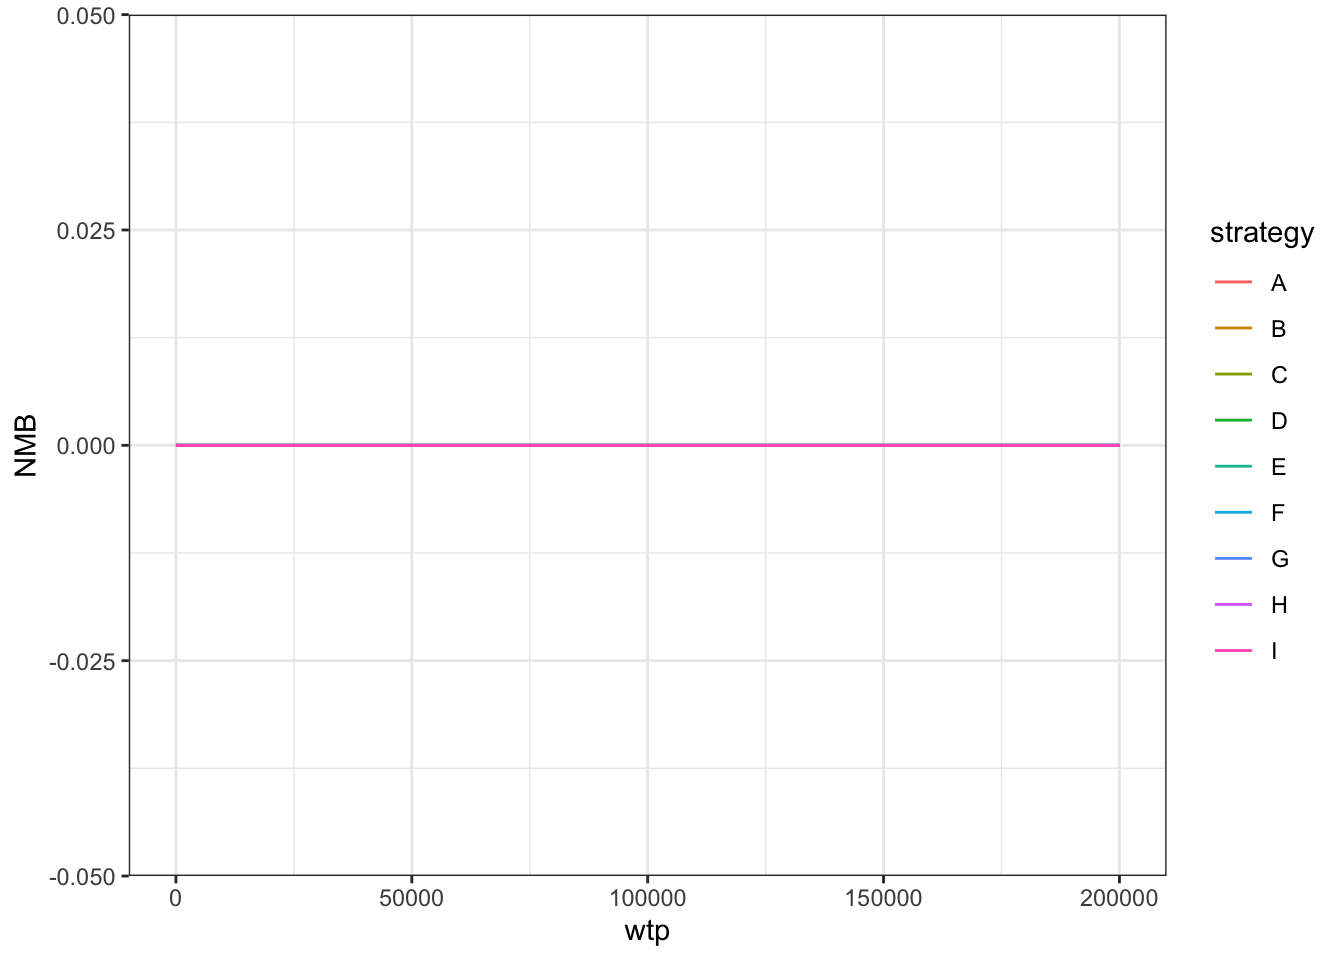
\includegraphics{assign1_trees_cea_files/figure-pdf/unnamed-chunk-12-1.pdf}

}

\end{figure}

Comparing the net monetary benefit plot to your incremental analysis
from the societal perspective, you should observe the following:

\begin{itemize}
\item
  All non-dominated interventions maximize net monetary benefit for some
  willingness-to-pay level (i.e., their line is the highest on the Y
  axis for some segment of the X axis).
\item
  The willingness-to-pay level at which we `flip' from preferring
  non-dominated strategy i to non-dominated strategy j can be derived
  from the NMB analysis or the incremental analysis:

  \begin{itemize}
  \item
    In incremental analysis, this corresponds to the ICER for
    intervention j vs.~i
  \item
    In the NMB plot, this corresponds to the WTP level (x-axis value) at
    which the line for strategy j crosses from below to above the line
    for strategy i.
  \end{itemize}
\end{itemize}

\hypertarget{last-two-questions}{%
\section{Last two questions}\label{last-two-questions}}

\begin{itemize}
\item
  About how much time did you spend on the assignment? \textbf{Replace
  with your answer}
\item
  Did you find any errors or have suggestions to improve it?
  \textbf{Replace with your answer}
\end{itemize}

Fin.



\end{document}
